\documentclass{beamer}

% Theme selection
\usetheme{Madrid}
\useoutertheme{miniframes}
\useinnertheme{circles}


\definecolor{UBCgreen}{rgb}{0.05, 0.4, 0.1}
\definecolor{UBCorange}{rgb}{1.0, 0.6, 0.0}
\definecolor{UBClightorng}{rgb}{1.0, 0.85, 0.3}
\definecolor{UBCdrkgry}{rgb}{0.3, 0.3, 0.3}

\usecolortheme[named=UBCgreen]{structure}

\setbeamercolor{frametitle}{fg=white,bg=UBCorange} 
\setbeamercolor{title}{fg=UBCorange} 
\setbeamercolor{block title}{fg=UBCdrkgry, bg=UBClightorng} 
\setbeamercolor{progress bar}{fg=UBCorange,bg=UBCgreen} 

% Packages
\usepackage[utf8]{inputenc}
\usepackage[ngerman]{babel}
\usepackage{graphicx}
\usepackage{hyperref}
\hypersetup{colorlinks=true}

\usepackage{caption}
\usepackage{multicol}
\usepackage{multirow}
\usepackage[dvipsnames]{xcolor}
\usepackage{pifont}
\usepackage{eurosym}
\usepackage{fontawesome}

\usepackage{tikz}
\usepackage{pgfplots}
\usepackage{pgfplotstable}
 
\usepackage{xcolor}
\usepackage{transparent}
\usepackage{siunitx}
\usepackage{array, dcolumn}

\usepackage{csquotes}

\usepackage[absolute,overlay]{textpos}

\usepackage[backend=biber]{biblatex}
\addbibresource{references.bib}

\title{§14a EnWG \- Steuerbare Verbraucher}
\author{Daniel Glaser}
\date{\today}

\newcommand{\grok}{\multirow{2}{*}{{\color{green}\ding{51}}}}
\newcommand{\rdno}{\multirow{2}{*}{{\color{red}\ding{55}}}}
\newcommand{\TimeBar}[1]{
   % Usage:   \TimeBar{<COLOR>/<START>/<END>, <COLOR>/<START>/<END>,...}
   % Examlpe: \TimeBar{green/0/5, yellow/5/17, red/17/21, yellow/21/24}
   \begin{tikzpicture}
      \def\totalwidth{2.5}
      \def\starttime{0}
      \def\endtime{24}
      \def\height{.2}

      \foreach \c/\start/\end in {#1} {
         \pgfmathsetmacro{\xstart}{(\start-\starttime)/(\endtime-\starttime)*\totalwidth}
         \pgfmathsetmacro{\xend}{(\end-\starttime)/(\endtime-\starttime)*\totalwidth}
         \fill[\c] (\xstart, 0) rectangle (\xend, \height);
      }

      \draw[black, very thin] (0, 0) rectangle (\totalwidth, \height);
      \foreach \dash in {6,12,18} {
         \pgfmathsetmacro{\xpos}{(\dash)/(\endtime)*\totalwidth}
         \draw[densely dotted, very thin] (\xpos,0) -- (\xpos,\height);
      }

   \end{tikzpicture}
}

\newcommand{\smp}{
\includegraphics[width=0.2cm]{images/party.png}}
\newcommand{\sml}{
\includegraphics[width=0.2cm]{images/lacheln.png}}
\newcommand{\smn}{
\includegraphics[width=0.2cm]{images/neutral.png}}
\newcommand{\sms}{
\includegraphics[width=0.2cm]{images/traurig.png}}

\begin{document}

% Titelseite
\begin{frame}
   \begin{tikzpicture}[remember picture, overlay]
      \node[at=(current page.center),opacity=0.1,yshift=-0.3cm]{
            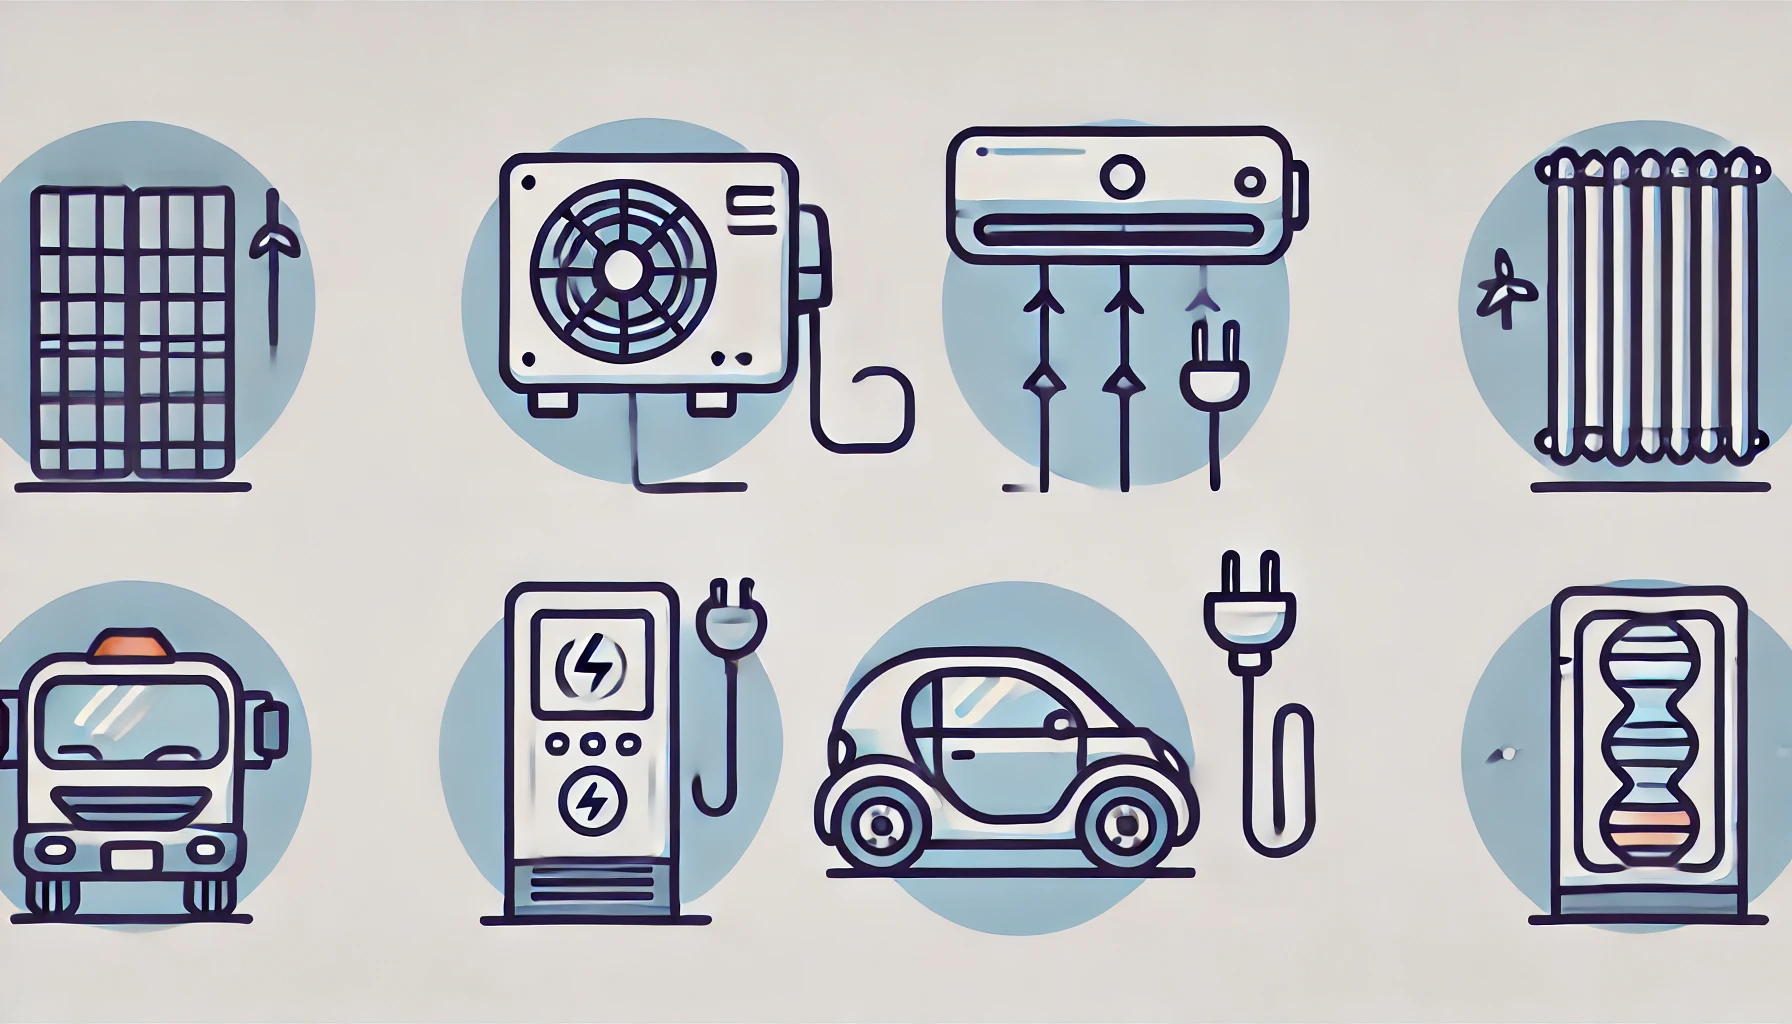
\includegraphics[height=0.9\paperheight]{images/Steuerbare_Verbraucher.png}
      };
   \end{tikzpicture}
   \titlepage
   \begin{textblock*}{3cm}(0.3cm,6.6cm)  % Position (x,y) in cm anpassen
      
\includegraphics[width=5cm]{images/Logo_EWERH_eV_small.png}
   \end{textblock*}
\end{frame}

% Inhaltsverzeichnis
\begin{frame}{Inhaltsverzeichnis}
   \tableofcontents
\end{frame}

%%%%%%%%%%%%%%%%%%%%%%%%
% Einführung in §14a   %
%%%%%%%%%%%%%%%%%%%%%%%%

\section{Einführung in §14a}

\begin{frame}[allowframebreaks]{Hintergrund}
    \begin{block}{Was ist §14a EnWG (Energie-Wirtschaftsgesetz)?}
        Der \href{https://www.gesetze-im-internet.de/enwg_2005/__14a.html}{§14a} des Energiewirtschaftsgesetzes (EnWG2024\cite{EnWG2024}) regelt die steuerbare Nutzung bestimmter elektrischer Verbraucher im Stromnetz. Ziel ist es, durch eine netzdienliche Steuerung der Lasten Engpässe im Stromnetz zu vermeiden und eine effizientere Nutzung erneuerbarer Energien zu ermöglichen.
        Zudem werden variable Netzentgelte eingeführt.
    \end{block}

    \framebreak

    \begin{block}{Warum sind steuerbare Verbraucher wichtig?}
        \begin{itemize}
            \item Vermeidung von Netzüberlastungen
            \item Förderung der Energiewende
            \item Kosteneinsparungen beim Netzausbau
        \end{itemize}
    \end{block}

    \begin{block}{Warum sind variable Netzentgelte wichtig?}
        \begin{itemize}
            \item Vermeidung von hohen Netzlasten
            \item Verschiebung von Lasten in Niederlastzeiten
            \item Bessere Auslastung der Netzte
            \item ...dadurch weitere Kosteneinsparungen beim Netzausbau
        \end{itemize}
    \end{block}

    \framebreak

    \begin{block}{Auswirkungen auf Haushalte}
        \begin{itemize}
            \item Kosteneinsparung durch Verbrauch in günstigen Zeiten
            \item Teils Veränderung des Nutzerverhaltens nötig
            \item Direkter Einfluss auf eigene Netzkosten
            \item Erst mit SmartHome bzw. Energy Manager optimal nutzbar
        \end{itemize}
    \end{block}
    \begin{block}{Auswirkungen auf Netzbetreiber}
        \begin{itemize}
            \item Bedarf an intelligenten Messsystemen wächst
            \item Anforderung an IT-Infrastruktur
            \item Entlastung beim Ausbaubedarf an Netzknoten und Netzen
            \item Zwangsweise Umstellung auf digitalisierte Prozesse
        \end{itemize}
    \end{block}
\end{frame}

\begin{frame}{Rechtliche Grundlagen - Bundesnatzagentur}
    \begin{block}{Beschluss BK8-22/010-A}
        In §14a EnWG \cite{EnWG2024} hat der Gesetzgeber festgelegt, dass Verteilnetzbetreiber künftig variable Netzentgelte für steuerbare Verbrauchseinrichtungen anbieten müssen. 
        Die Pflicht zur genauen Festlegung wurde der Bundesnatzagentur übertragen, 
        welche bereits am 23.11.2023 den Beschluss BK8-22/010-A\cite{BNetzA-BK8-22-010-A} fasste.
    \end{block}
\end{frame}
   
\begin{frame}{Rechtliche Grundlagen - Beschluss BK8-22/010-A}

   Im Beschluss BK8-22/010-A\cite{BNetzA-BK8-22-010-A} der Bundesnetzagentur ist festgelegt, dass...
   \vspace{0.5cm}
   \begin{description}
      \item[Modul 1] eine jährliche Erstattung,
      \item[Modul 2] einen ermäßigten Tarif,
      \item[Modul 3] und ein variables Netzentgelt
   \end{description}
   \vspace{0.5cm}
   ...vom Netzbetreiber angeboten werden muss. 
\end{frame}
   
\begin{frame}{Rechtliche Grundlagen - Auswahl der Module}
    Hierbei kann/muss man wählen zwischen:
    \begin{description}
        \item[Modul 2] mit gesonderter Messung und reduziertem Arbeitspreis
        \item[Modul 1] mit pauschler Erstattung
        \item[Modul 1 \& 3] ...zusätzlich mit variablen Netzentgelten
    \end{description} 
    \vspace{0.5cm}
    \begin{block}{Festlegungen zur Ausgestaltung}    
        Hierbei wurden auch Festlegungen speziell zur Ausgestaltung des Moduls 3 getroffen bzgl. der Hoch- und 
        Niedertarifpreise und mindestens zweier Quartale (S.4 Abs.3c) pro Jahr mit variablen Netzentgelten.
    \end{block}
\end{frame}

\begin{frame}{Rechtliche Grundlagen - Vorgaben Modul 3}
   
   In der Anlage zum Beschluss (S.62) finden sich dann auch Details zur Tarifgestaltung.

   \begin{enumerate}
      \item Die Hochtarifstufe muss in mindestens zwei Stunden eines Tages abgerechnet werden 
         und darf die Standardtarifstufe um maximal 100\% übersteigen.
      \item Der Netzbetreiber hat eine Niedrigtarifstufe im Korridor zwischen 10 und 40\% der 
         Standardtarifstufe zu bilden.
      \item Ein hypothetischer Verbraucher mit einem dem Standardlastprofil für 
         Haushaltskunden (H0) identischen Verbrauchsprofil wäre bei einer existierenden 
         Wahlmöglichkeit indifferent zwischen dem Arbeitspreis für Entnahme ohne 
         Leisstungsmessung und dem Modul 3.
   \end{enumerate}
\end{frame}

\begin{frame}{Ergänzung - Haushaltslastprofil H0}
    \centering
    \begin{tikzpicture}
        \node[anchor=center] at (0, 0) {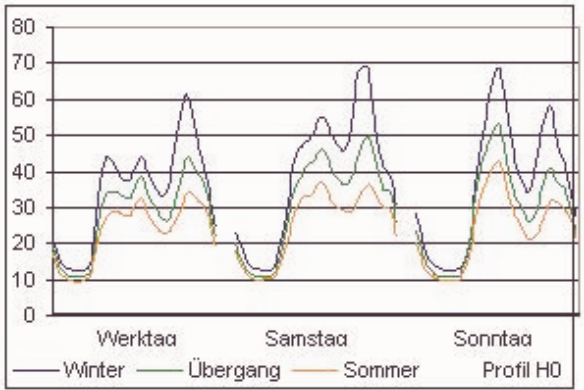
\includegraphics[height=0.70\paperheight]{images/Lastprofil_Haushalt_H0.png}};
        \node[rotate=90,anchor=center] at (5.5, 0) {Quelle: BDEW\cite{BDEW1999ReprLProf}};
    \end{tikzpicture}
 \end{frame}

 \begin{frame}{Stromerzeugung und Last - Winter}
    \centering
    \begin{tikzpicture}
        \node[anchor=center] at (0, 0) {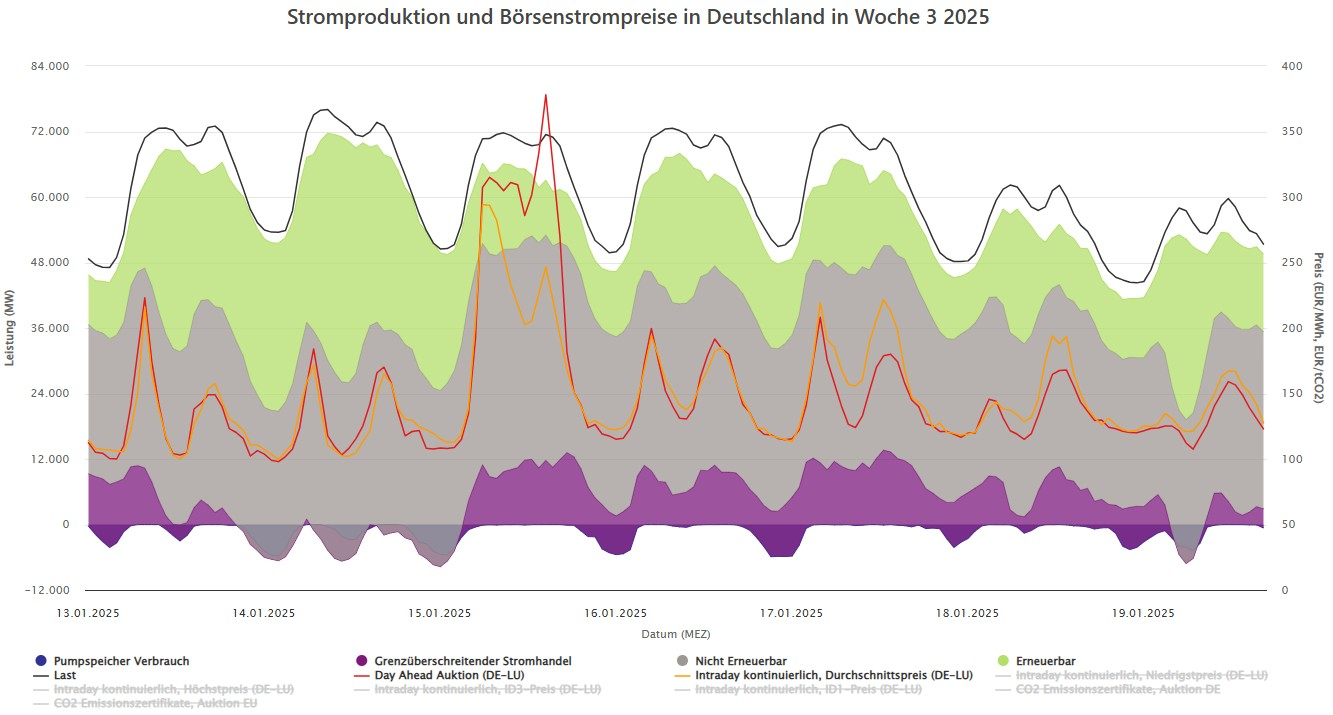
\includegraphics[width=0.9\paperwidth]{images/Stromproduktion_Winter.jpg}};
        \node[rotate=90,anchor=center] at (6, 0) {\tiny Quelle: Energy Charts};
    \end{tikzpicture}
\end{frame}

\begin{frame}{Stromerzeugung und Last - Frühling}
    \centering
    \begin{tikzpicture}
        \node[anchor=center] at (0, 0) {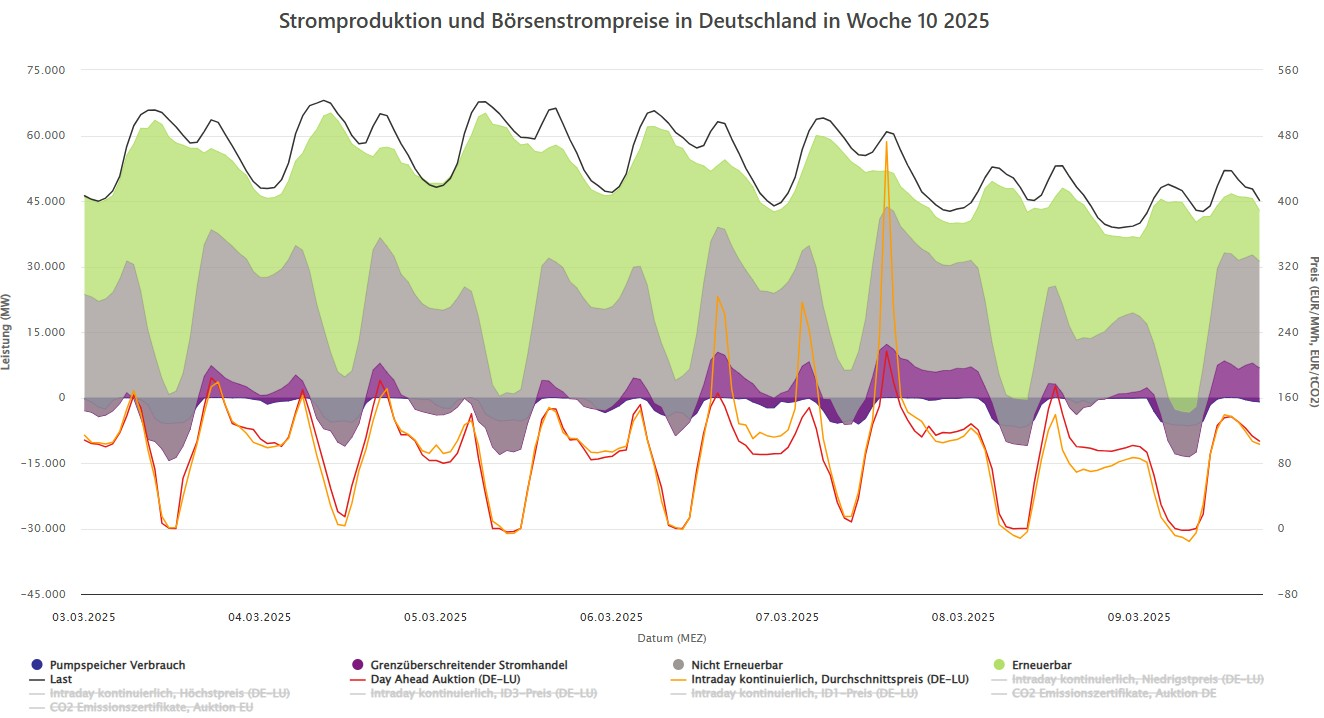
\includegraphics[width=0.9\paperwidth]{images/Stromproduktion_Fruehling.jpg}};
        \node[rotate=90,anchor=center] at (6, 0) {\tiny Quelle: Energy Charts};
    \end{tikzpicture}
\end{frame}

\begin{frame}{Stromerzeugung und Last - Sommer}
    \centering
    \begin{tikzpicture}
        \node[anchor=center] at (0, 0) {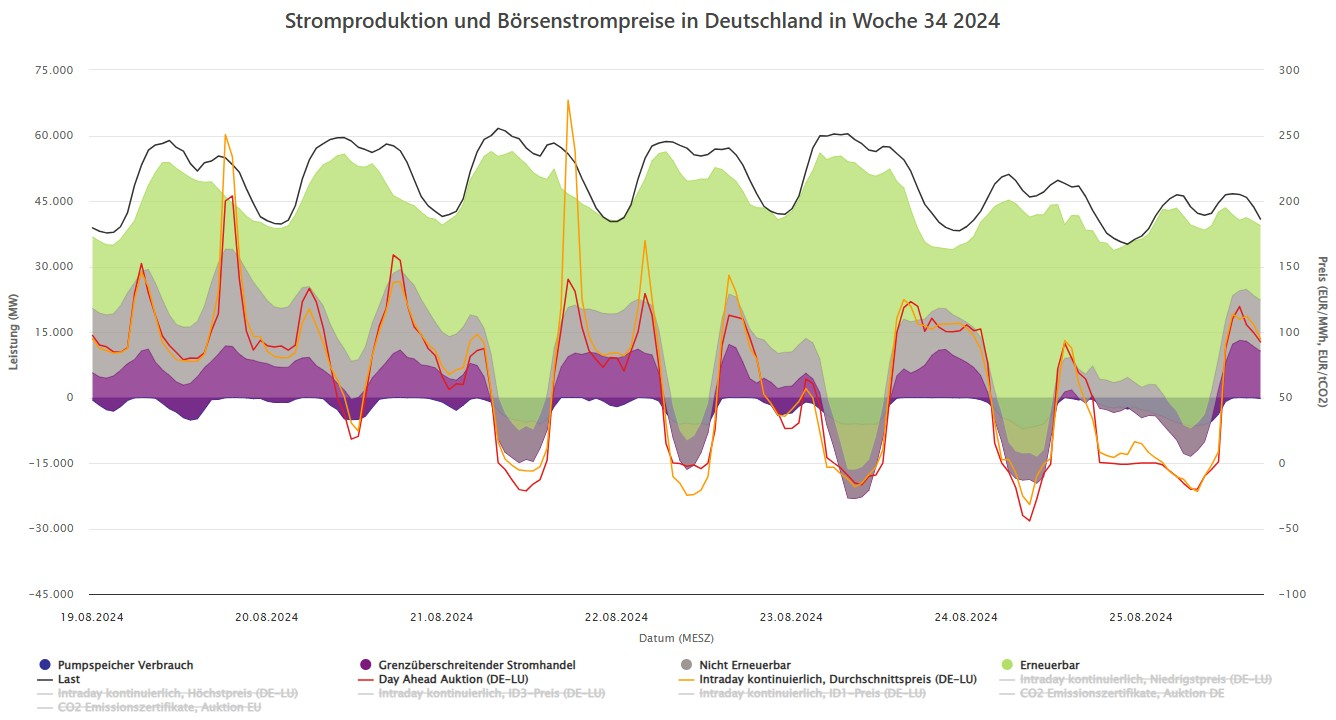
\includegraphics[width=0.9\paperwidth]{images/Stromproduktion_Sommer.jpg}};
        \node[rotate=90,anchor=center] at (6, 0) {\tiny Quelle: Energy Charts};
    \end{tikzpicture}
\end{frame}

%%%%%%%%%%%%%%%%%%%%%%%%%%
% Technische Umsetzung   %
%%%%%%%%%%%%%%%%%%%%%%%%%%
\section{Technische Umsetzung}

\begin{frame}{Intelligentes Messsystem - iMSys I}
   \begin{center}
      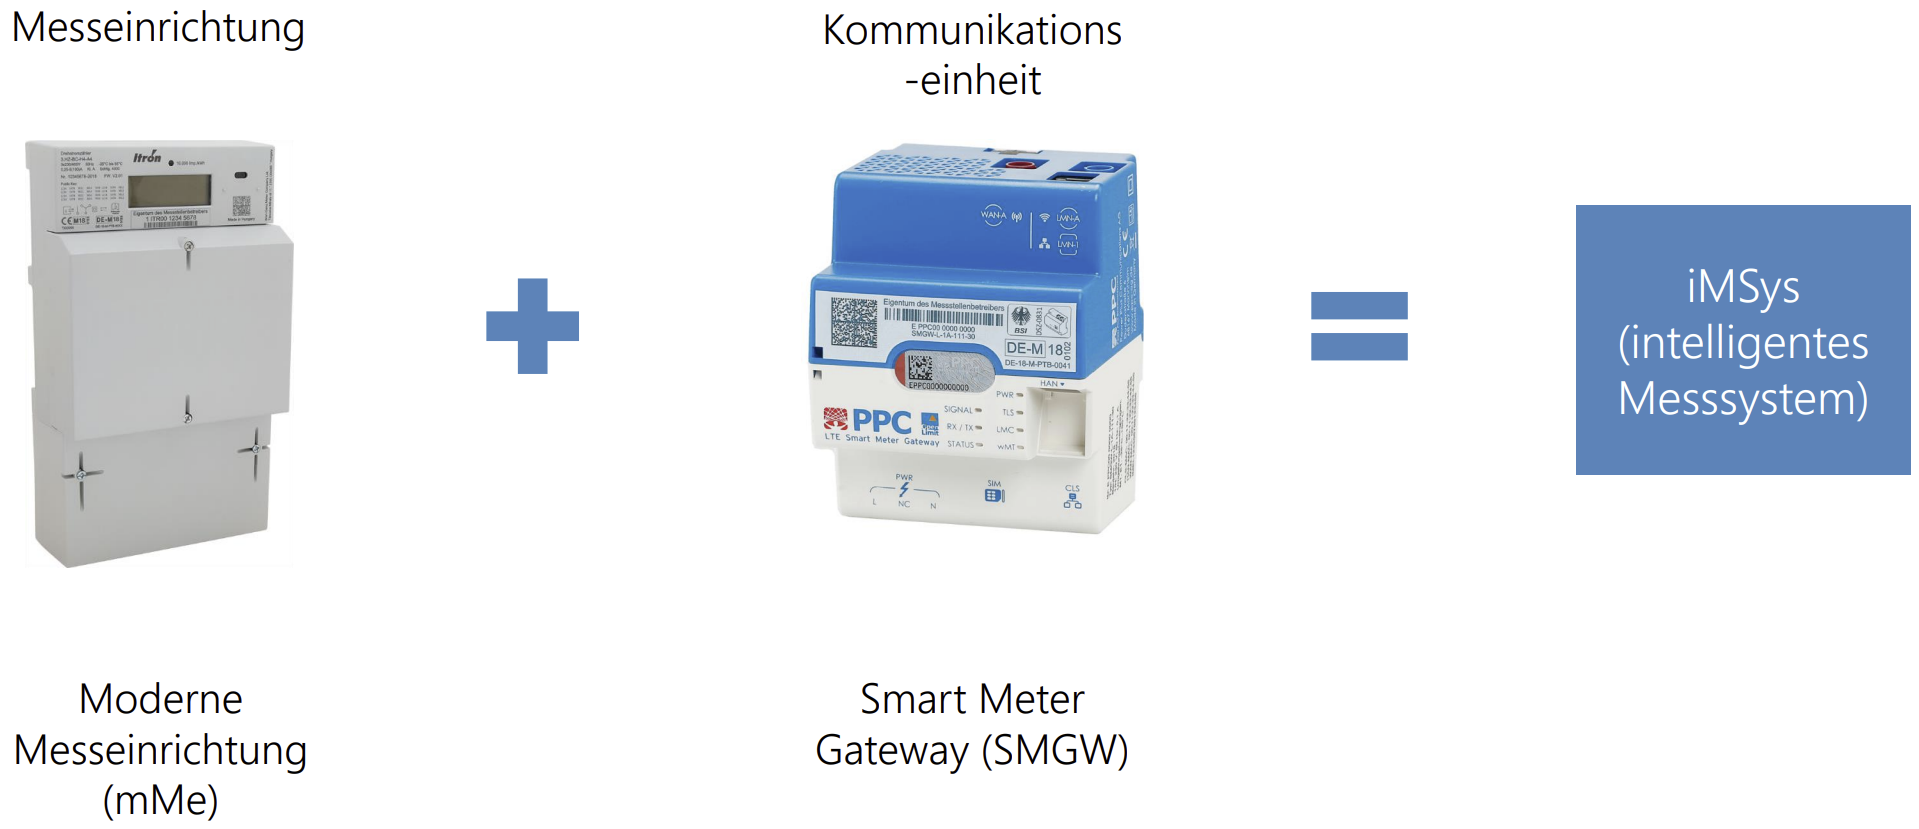
\includegraphics[width=10cm]{images/iMSys.png}
   \end{center}
   Quelle: FfE e.V.\cite{FFE2020imsys}
\end{frame}

\begin{frame}{Intelligentes Messsystem - iMSys II}
   \begin{center}
      \begin{minipage}{0.34\textwidth}
         \centering
         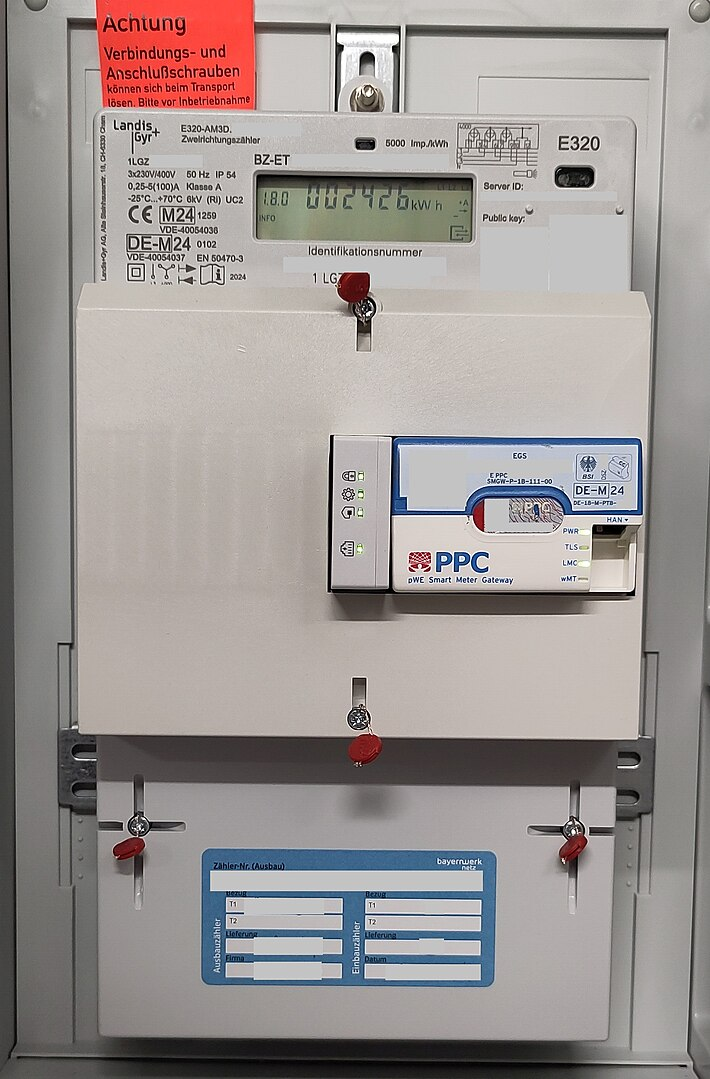
\includegraphics[width=\linewidth]{images/SmartMeter.jpg}
      \end{minipage}
      \begin{minipage}{0.64\textwidth}
         \centering
         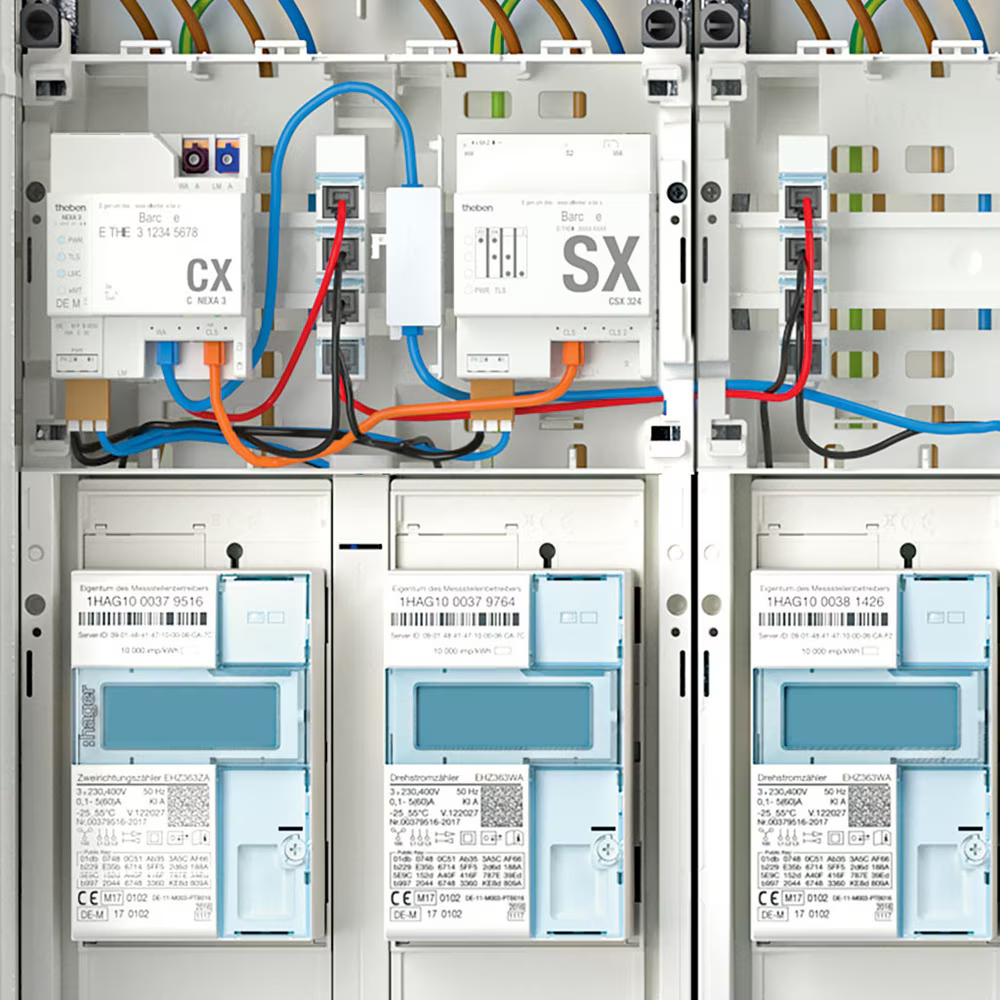
\includegraphics[width=0.8\linewidth]{images/technikzentrale.png}
      \end{minipage}
   \end{center}
   Quellen: \href{https://commons.wikimedia.org/wiki/File:2024-SmartMeter.jpg}{Wikipedia}, Hager
\end{frame}

\begin{frame}{Smart Meter Gateway}
   \begin{center}
      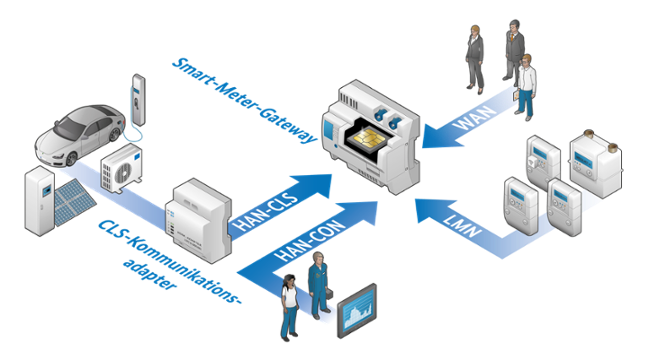
\includegraphics[width=10cm]{images/smartmetergateway.png}
   \end{center}
   Quelle: BSI\cite{FFE2020imsys}
   ,Detailinfos zu HAN VDE FNN\cite{VDEFNNimpulsDigitaleSchnittstellen2023}
\end{frame}

\begin{frame}{Zertifizierte Komponenten}
   \begin{itemize}
      \item TR-03109-1 \href{https://www.bsi.bund.de/DE/Themen/Unternehmen-und-Organisationen/Standards-und-Zertifizierung/Smart-metering/Smart-Meter-Gateway/Zertifikate24Msbg/produkte.html}{Smart-Meter-Gateways - SmGW} (13)
      \item TR-03109-5 \href{https://www.bsi.bund.de/DE/Themen/Unternehmen-und-Organisationen/Standards-und-Zertifizierung/Smart-metering/Kommunikationsadapter/Zertifikate/Zertifikate_TR_03109-5_node.html}{Steuerboxen - CLS} (8)
   \end{itemize}
   \vspace{0.3cm}
   \begin{center}
      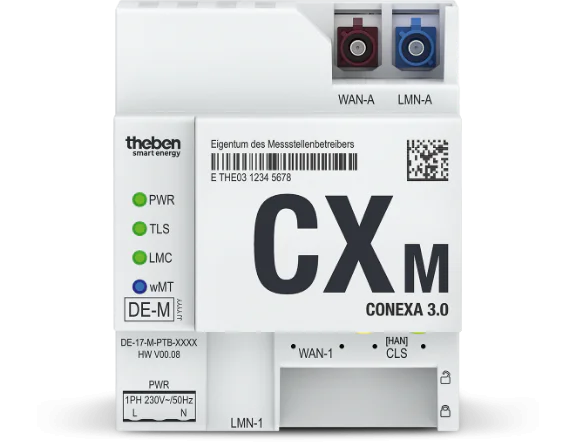
\includegraphics[height=4cm]{images/Theben_CXm.png}
      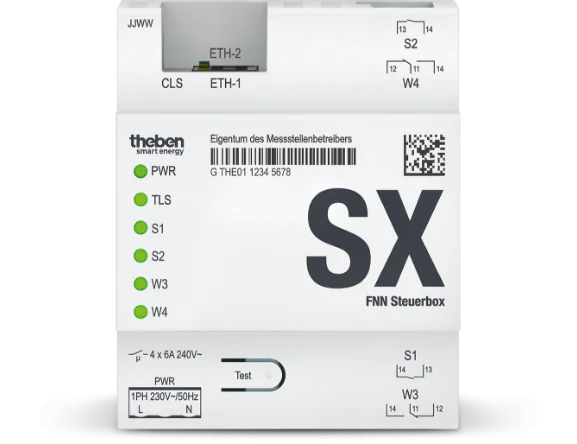
\includegraphics[height=4cm]{images/Theben_SX.png}
   \end{center}
\end{frame}

\begin{frame}{Netzdienliche Steuerung}
   \begin{block}{\enquote{Dimmen} von Verbrauchern $>4,2\,\text{kW}$}
      \begin{itemize}         
         \item Begrenzung der elektrischen Leistung auf 4,2 kW...
         \item ...Wärmepumpen z.B. Heizstab deaktivieren (SG-Ready)
         \item ...Wallbox teilt Maximalleistung 4,2 kW mit (PWM-Signal)
         \item ...Speicher Netzbezug auf 4,2 kW drosseln
      \end{itemize}
   \end{block}
   \begin{block}{Verbraucher mittels Preissignalen steuern}
      \begin{itemize}
         \item Fixe Zeitfenster mit drei Netzentgeltstufen
         \item Laden des E-Autos in Schwachlastzeiten
         \item Bevorzugt laden des Speichers in Schwachlastzeiten
         \item Entladen des Speichers in Hochlastzeiten
         \item Heizungspuffer \enquote{füllen} + Warmwasserbereitung
      \end{itemize}
   \end{block}
   \vspace{0.3cm}
\end{frame}

\begin{frame}
   \frametitle{Roll-Out Quoten Q4/2024}
   \centering
   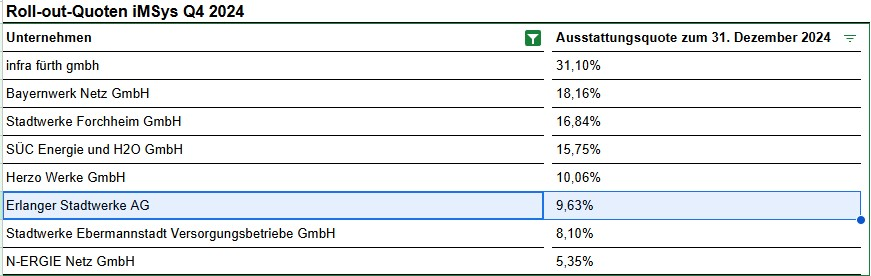
\includegraphics[width=0.95\paperwidth]{images/Roll-Out-Quoten.jpg}
\end{frame}


%%%%%%%%%%%%%%%%%%%%%%%%%%%
% Wirtschaftliche Aspekte %
%%%%%%%%%%%%%%%%%%%%%%%%%%%
\section{Wirtschaftliche Aspekte}

\begin{frame}{Kosten und Nutzen I}
    \centering
    Variabler Strompreis (2025-03-06)
    \begin{tikzpicture}
        \begin{axis}[
            width=12cm, height=7cm, % Größe des Plots
            xlabel={Uhrzeit (h)}, % Beschriftung X-Achse
            ylabel={Preis (ct/kWh)}, % Beschriftung Y-Achse
            xtick={0,3,6,9,12,15,18,21,24}, % Markierungen auf der X-Achse
            ymin=0, ymax=65, % Wertebereich für die Preise
            xticklabel style={anchor=north}, % Ausrichtung der X-Achsen-Beschriftung
            yticklabel style={anchor=east}, % Ausrichtung der Y-Achsen-Beschriftung
            grid=major, % Gitterlinien
            enlargelimits=false, % Begrenzung der Achsen direkt an den Rändern
            domain=0:24,
            legend pos=north west,
            legend style={font=\footnotesize},
            legend cell align=left
        ]
        
        \addplot[thick, red, mark=*] coordinates {
            (0.5, 29) (1.5, 29.2) (2.5, 29.4) (3.5, 29.5) 
            (4.5, 30.3) (5.5, 30.5) (6.5, 35.6) (7.5, 37.1) 
            (8.5, 32) (9.5, 28.4) (10.5, 25.1) (11.5, 19.5) 
            (12.5, 19.1) (13.5, 19.1) (14.5, 20.6) (15.5, 27.5) 
            (16.5, 32.9) (17.5, 36.8) (18.5, 38.7) (19.5, 36.8) 
            (20.5, 34) (21.5, 31.8) (22.5, 31.1) (23.5, 29.9) 
        };
        \addlegendentry{Tibber}
        
        % \pgfmathsetmacro{\vntsub}{\vst-\vnt}
        % \pgfmathsetmacro{\vhtadd}{\vht-\vst}

        % %NT:  0.75 ->  0.8925 (netto)
        % %ST:  7.52 ->  9.9488 (netto)
        % %HT: 14.26 -> 16.9694 (netto)
        % \addplot[thick, ForestGreen, mark=triangle, opacity = 0.8] coordinates {
        %     (0.5, 31.17 - \vntsub) (1.5, 30.97- \vntsub) 
        %     (2.5, 30.70- \vntsub) (3.5, 30.65 - \vntsub) 
        %     (4.5, 31.18 - \vntsub) (5.5, 32.19 - \vntsub) 
        %     (6.5, 36.26) (7.5, 38.30) (8.5, 36.72) (9.5, 33.94) (10.5, 31.27)
        %     (11.5, 30.92 + \vhtadd) (12.5, 30.73 + \vhtadd) 
        %     (13.5, 30.95) (14.5, 31.16) (15.5, 33.07) (16.5, 35.97) 
        %     (17.5, 37.75 + \vhtadd) (18.5, 42.83 + \vhtadd) 
        %     (19.5, 40.42) (20.5, 36.68) (21.5, 34.79) 
        %     (22.5, 33.34 - \vntsub) (23.5, 32.14 - \vntsub) 
        % };
        % \addlegendentry{ESTW VNB + Tibber}
        
        \end{axis}
    \end{tikzpicture}
\end{frame}

\begin{frame}{Kosten und Nutzen II}
    Var. Netzentgelte vs. dyn. Strompreis (Übergang 2025-03-12)
    \begin{tikzpicture}
        \begin{axis}[
            width=12cm, height=7cm, % Größe des Plots
            xlabel={Uhrzeit (h)}, % Beschriftung X-Achse
            ylabel={Preis (ct/kWh)}, % Beschriftung Y-Achse
            xtick={0,3,6,9,12,15,18,21,24}, % Markierungen auf der X-Achse
            ymin=0, ymax=65, % Wertebereich für die Preise
            xticklabel style={anchor=north}, % Ausrichtung der X-Achsen-Beschriftung
            yticklabel style={anchor=east}, % Ausrichtung der Y-Achsen-Beschriftung
            grid=major, % Gitterlinien
            enlargelimits=false, % Begrenzung der Achsen direkt an den Rändern
            domain=0:24,
            legend pos=north west,
            legend style={font=\footnotesize},
            legend cell align=left
        ]
        
        % Beispiel: Balkendiagramm für stündliche Preise
        \pgfmathsetmacro{\vnt}{0.75*1.19}
        \pgfmathsetmacro{\vst}{7.52*1.19}
        \pgfmathsetmacro{\vht}{14.26*1.19}

        \addplot[ybar, fill=blue!30] coordinates {
            (0.5, \vnt) (1.5, \vnt) (2.5, \vnt) (3.5, \vnt) (4.5, \vnt) 
            (5.5, \vnt) (6.5, \vst) (7.5, \vst) (8.5, \vst) (9.5, \vst) 
            (10.5, \vst) (11.5, \vht) (12.5, \vht) (13.5, \vst) (14.5, \vst) 
            (15.5, \vst) (16.5, \vst) (17.5, \vht) (18.5, \vht) (19.5, \vnt) 
            (20.5, \vnt) (21.5, \vnt) (22.5, \vnt) (23.5, \vnt) 
        };
        \addlegendentry{ESTW VNE}
    
        % Alternative: Liniengrafik
        \addplot[thick, red, mark=*] coordinates {
            (0.5, 31.17) (1.5, 30.97) (2.5, 30.70) (3.5, 30.65) 
            (4.5, 31.18) (5.5, 32.19) (6.5, 36.26) (7.5, 38.30) 
            (8.5, 36.72) (9.5, 33.94) (10.5, 31.27) (11.5, 30.92) 
            (12.5, 30.73) (13.5, 30.95) (14.5, 31.16) (15.5, 33.07) 
            (16.5, 35.97) (17.5, 37.75) (18.5, 42.83) (19.5, 40.42) 
            (20.5, 36.68) (21.5, 34.79) (22.5, 33.34) (23.5, 32.14) 
        };
        \addlegendentry{Tibber}
        
        \pgfmathsetmacro{\vntsub}{\vst-\vnt}
        \pgfmathsetmacro{\vhtadd}{\vht-\vst}

        %NT:  0.75 ->  0.8925 (netto)
        %ST:  7.52 ->  9.9488 (netto)
        %HT: 14.26 -> 16.9694 (netto)
        \addplot[thick, ForestGreen, mark=triangle, opacity = 0.8] coordinates {
            (0.5, 31.17 - \vntsub) (1.5, 30.97- \vntsub) 
            (2.5, 30.70- \vntsub) (3.5, 30.65 - \vntsub) 
            (4.5, 31.18 - \vntsub) (5.5, 32.19 - \vntsub) 
            (6.5, 36.26) (7.5, 38.30) (8.5, 36.72) (9.5, 33.94) (10.5, 31.27)
            (11.5, 30.92 + \vhtadd) (12.5, 30.73 + \vhtadd) 
            (13.5, 30.95) (14.5, 31.16) (15.5, 33.07) (16.5, 35.97) 
            (17.5, 37.75 + \vhtadd) (18.5, 42.83 + \vhtadd) 
            (19.5, 40.42 - \vntsub) (20.5, 36.68 - \vntsub) 
            (21.5, 34.79 - \vntsub) 
            (22.5, 33.34 - \vntsub) (23.5, 32.14 - \vntsub) 
        };
        \addlegendentry{ESTW VNB + Tibber}
        
        \end{axis}
    \end{tikzpicture}
\end{frame}

\begin{frame}{Kosten und Nutzen III}
    Var. Netzentgelte vs. dyn. Strompreis (Sommer, 2024-07-06)
    \begin{tikzpicture}
        \begin{axis}[
            width=12cm, height=7cm, % Größe des Plots
            xlabel={Uhrzeit (h)}, % Beschriftung X-Achse
            ylabel={Preis (ct/kWh)}, % Beschriftung Y-Achse
            xtick={0,3,6,9,12,15,18,21,24}, % Markierungen auf der X-Achse
            ymin=0, ymax=65, % Wertebereich für die Preise
            xticklabel style={anchor=north}, % Ausrichtung der X-Achsen-Beschriftung
            yticklabel style={anchor=east}, % Ausrichtung der Y-Achsen-Beschriftung
            grid=major, % Gitterlinien
            enlargelimits=false, % Begrenzung der Achsen direkt an den Rändern
            domain=0:24,
            legend pos=north west,
            legend style={font=\footnotesize},
            legend cell align=left
        ]
        
        % Beispiel: Balkendiagramm für stündliche Preise
        \pgfmathsetmacro{\vnt}{0.75*1.19}
        \pgfmathsetmacro{\vst}{7.52*1.19}
        \pgfmathsetmacro{\vht}{14.26*1.19}

        \addplot[ybar, fill=blue!30] coordinates {
            (0.5, \vnt) (1.5, \vnt) (2.5, \vnt) (3.5, \vnt) (4.5, \vnt) 
            (5.5, \vnt) (6.5, \vst) (7.5, \vst) (8.5, \vst) (9.5, \vst) 
            (10.5, \vst) (11.5, \vht) (12.5, \vht) (13.5, \vst) (14.5, \vst) 
            (15.5, \vst) (16.5, \vst) (17.5, \vht) (18.5, \vht) (19.5, \vnt) 
            (20.5, \vnt) (21.5, \vnt) (22.5, \vnt) (23.5, \vnt) 
        };
        \addlegendentry{ESTW VNE}
    
        % Alternative: Liniengrafik
        \addplot[thick, red, mark=*] coordinates {
            (0.5, 27.2) (1.5, 25) (2.5, 24.2) (3.5, 22.1) 
            (4.5, 21.2) (5.5, 18.5) (6.5, 17.3) (7.5, 17.2) 
            (8.5, 17) (9.5, 16.6) (10.5, 15.4) (11.5, 13.2) 
            (12.5, 12.7) (13.5, 11.4) (14.5, 10.9) (15.5, 12.5) 
            (16.5, 15) (17.5, 16.6) (18.5, 16.8) (19.5, 16.6) 
            (20.5, 17.4) (21.5, 17.7) (22.5, 18.8) (23.5, 18.3) 
        };
        \addlegendentry{Tibber}
        
        \pgfmathsetmacro{\vntsub}{\vst-\vnt}
        \pgfmathsetmacro{\vhtadd}{\vht-\vst}

        %NT:  0.75 ->  0.8925 (netto)
        %ST:  7.52 ->  9.9488 (netto)
        %HT: 14.26 -> 16.9694 (netto)
        \addplot[thick, ForestGreen, mark=triangle, opacity = 0.8] coordinates {
            (0.5, 27.2 - \vntsub) (1.5, 25 - \vntsub) 
            (2.5, 24.2 - \vntsub) (3.5, 22.1 - \vntsub) 
            (4.5, 21.2 - \vntsub) (5.5, 18.5 - \vntsub) 
            (6.5, 17.3) (7.5, 17.2) (8.5, 17) (9.5, 16.6) (10.5, 15.4) 
            (11.5, 13.2 + \vhtadd) (12.5, 12.7 + \vhtadd) 
            (13.5, 11.4) (14.5, 10.9) (15.5, 12.5) (16.5, 15) 
            (17.5, 16.6 + \vhtadd) (18.5, 16.8 + \vhtadd) 
            (19.5, 16.6 - \vntsub) (20.5, 17.4 - \vntsub) 
            (21.5, 17.7 - \vntsub) 
            (22.5, 18.8 - \vntsub) (23.5, 18.3 - \vntsub) 
        };
        \addlegendentry{ESTW VNB + Tibber}
        
        \end{axis}
    \end{tikzpicture}

\end{frame}

\begin{frame}{Beispielrechnungen (ESTW)}
    \begin{center}        
        \begin{tabular}{l c | S[table-format=2.2] c S[table-format=2.4]}
            \multicolumn{2}{c|}{\textbf{Tarif}} 
              & \multicolumn{1}{c}{\textbf{netto (ct/kWh)}} 
              & \multicolumn{1}{c}{} 
              & \multicolumn{1}{c}{\textbf{brutto (ct/kWh)}} \\\hline
            Niedertarif   & NT & 0.75  & → & 0.8925  \\
            Standardtarif & ST & 7.52  & → & 9.9488  \\
            Hochtarif     & HT & 14.26 & → & 16.9694
        \end{tabular}
           
    \end{center}

    % \begin{description}
    %     \item[WP] 10 kW\textsubscript{th}, 3 kW\textsubscript{el}: $\approx 9$ ct/h $\rightarrow$ 180 \EUR{}/a
    %     \item[Speicher] 10 kWh $\rightarrow$ $\approx 80$ ct/d, 200 d/a $\rightarrow$ 160 \EUR{}/a
    %     \item[E-Auto] 15 tkm, 60\%@\faHome, 17 kWh/100 km, $\approx 9$ ct/kWh $\rightarrow$ 140 \EUR{}/a
    % \end{description}

    \begin{tabular}{l l c l}
        \textbf{Was?} & \textbf{Annahmen} & \textbf{Einsparung} & \textbf{Jährlich} \\
        \hline
        WP       & \SI{10}{kW_{\text{th}}}, \SI{3}{kW_{\text{el}}}, 2000 h/a & $\approx$ 9 ct/h  & 180\EUR{}/a \\

        Speicher & \SI{10}{kWh}, 200 d/a & $\approx$ 80 ct/d & 160\EUR{}/a \\

        E-Auto   & \SI{15}{tkm}, 60\%@\faHome, \SI{17}{kWh/100km} & $\approx$ 9 ct/kWh  & 140\EUR{}/a \\
    \end{tabular}

    \begin{block}{Flexibilität als Schlüssel mit Einschränkungen}
        Durch Lastverschiebungen sind diese Einsparungen mit VNE gut erreichbar. Dynamische Strompreise sind schlechter kalkulierbar und stark abhängig davon, wie gut und lange man die Last verschieben kann.
    \end{block}

\end{frame}


%%%%%%%%%%%%%%%%%%%%%%%%%
% Regionales            %
%%%%%%%%%%%%%%%%%%%%%%%%%
\section{Regionales}

\begin{frame}{Verteilnetzbetreiber}
   \begin{columns}
      % Linke Spalte für das Bild
      \column{0.70\textwidth}
      \centering
      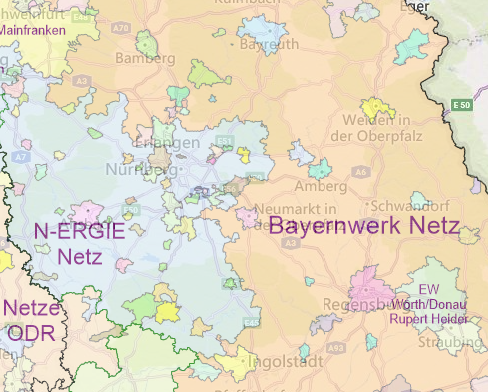
\includegraphics[width=\linewidth]{images/Verteilnetzbetreiber_Umland_ERH.png}

      % Rechte Spalte für die Item-Liste
      \column{0.3\textwidth}
      Netzgesellschaften:
      \begin{itemize}
         \item \href{https://netze.estw.de/}{ESTW}
         \item \href{https://www.bayernwerk-netz.de/de.html}{Bayernwerk}
         \item \href{https://www.herzowerke.de/de/netz/stromnetz/}{Herzo-Werke}
         \item \href{https://www.n-ergie-netz.de/}{N-ERGIE}
         \item \href{https://www.stadtwerke-ebermannstadt.de/de/Kopfnavigation/Netze1/Stromnetz/}{Ebermannstadt}
         \item \href{https://www.stadtwerke-forchheim.de/}{Forchheim}
         \item \href{https://www.suec-netze.de/}{SÜC}
      \end{itemize}
      Bildquelle: \href{https://www.netze-und-versorger.de/}{infas360}
   \end{columns}
\end{frame}

\begin{frame}{Kurzübersicht Netzbetreiber}
   \begin{table}[h]
      \centering
      % !TeX indents-off
      {\tiny
         \begin{tabular}{|l|cccc|c|c|ccc|}
            \hline
            \textbf{VNB} & \textbf{Q1} & \textbf{Q2} & \textbf{Q3} & \textbf{Q4} 
            & \textbf{M1 (\EUR{}/a)} & \textbf{M2 (ct/kWh)} & \multicolumn{3}{c|}{\textbf{M3 (ct/kWh)}} \\\hline
   
            \multirow{3}{*}{\smp\ ESTW\cite{estwnetznutz2025}}
              & \grok & \grok & \grok & \grok & \multirow{3}{*}{123,63 \smn} & \multirow{3}{*}{3,01 \sml} & NT & 22-6h             &  0,75 \\
              &       &       &       &       &                         &  & ST & 6-11,13-17,19-22h &  7,52 \\
              & \multicolumn{4}{c|}{\TimeBar{green/0/6, yellow/6/11, red/11/13, yellow/13/17, red/17/19, yellow/19/22, green/22/24}}
                                              &                         &  & HT & 11-13,17-19h      & 14,26 \\\hline

            
            \multirow{3}{*}{\sml\ Bayernwerk\cite{bayernwerknetznutz2025}} 
              & \grok & \rdno & \rdno & \grok & \multirow{3}{*}{122,35 \smn} & \multirow{3}{*}{2,94 \sml} & NT & 0-5h              &  0,74 \\
              &       &       &       &       &                         &  & ST & 5-17,21-0h        &  7,35 \\
              & \multicolumn{4}{c|}{\TimeBar{green/0/5, yellow/5/17, red/17/21, yellow/21/24}} 
                                              &                         &  & HT & 17-21h            &  9,72 \\\hline
            
            \multirow{3}{*}{\sml\ HerzoWerke\cite{herzowerkenetznutz2025}} 
              & \grok & \rdno & \rdno & \grok & \multirow{3}{*}{165,48 \smp} & \multirow{3}{*}{5,24 \sms} & NT & 0-6h              &  3,28 \\
              &       &       &       &       &                         &  & ST & 6-11,12-16,20-0h  & 13,10 \\
              & \multicolumn{4}{c|}{\TimeBar{green/0/6, yellow/6/11, red/11/12, yellow/12/16, red/16/20, yellow/20/24}} 
                                              &                         &  & HT & 11-12,16-20h      & 17,04 \\\hline
         
            \multirow{3}{*}{\smn\ N-ERGIE\cite{nergienetznutz2025}} 
              & \grok & \rdno & \rdno & \grok & \multirow{3}{*}{115,08 \sms} & \multirow{3}{*}{2,55 \smp} & NT & 23-7h             &  0,64 \\
              &       &       &       &       &                         &  & ST & 7-18,21-23h       &  6,38 \\
              & \multicolumn{4}{c|}{\TimeBar{green/0/7, yellow/7/18, red/18/21, yellow/21/23, green/23/24}} 
                                              &                         &  & HT & 18-21h            & 11,85 \\\hline
   
            \multirow{3}{*}{\sml\ Ebermannst.\cite{ebermannstadtnetznutz2025}} 
              & \grok & \rdno & \rdno & \grok & \multirow{3}{*}{163,31 \smp} & \multirow{3}{*}{5,12 \sms} & NT & 22-6h             &  2,56 \\
              &       &       &       &       &                         &  & ST & 6-17,21-22h       & 12,81 \\
              & \multicolumn{4}{c|}{\TimeBar{green/0/6, yellow/6/17, red/17/21, yellow/21/22, green/22/24}} 
                                              &                         &  & HT & 17-21h            & 21,07 \\\hline
   
              \multirow{3}{*}{\sml\ Forchheim\cite{forchheimnetznutz2025}} 
              & \grok & \rdno & \rdno & \grok & \multirow{3}{*}{141,26 \sml} & \multirow{3}{*}{3,95 \smn} & NT & 0-6h              &  1,97 \\
              &       &       &       &       &                         &  & ST & 6-17,21-0h        &  9,87 \\
              & \multicolumn{4}{c|}{\TimeBar{green/0/6, yellow/6/17, red/17/21, yellow/21/24}} 
                                              &                         &  & HT & 17-21h            & 13,43 \\\hline
            
            \multirow{3}{*}{\sms\ SÜC\cite{suecnetznutz2025}} 
              & \rdno & \grok & \grok & \rdno & \multirow{3}{*}{122,73 \smn} & \multirow{3}{*}{2,96 \sml} & NT & 10-14h            &  1,82 \\
              &       &       &       &       &                         &  & ST & 22-10,14-17h      &  7,40 \\
              & \multicolumn{4}{c|}{\TimeBar{yellow/0/10, green/10/14, yellow/14/17, red/17/22, yellow/22/24}} 
                                              &                         &  & HT & 17-22h & 11,84 \\\hline
            
         \end{tabular}
      }
      \caption{Verteilnetzbetreiber in der Region Erlangen}
      \label{tab:verteilnetzbetreiber}
   \end{table}
\end{frame}

\begin{frame}{ESTW}
   \begin{textblock*}{3.3cm}(9.4cm,2cm)
      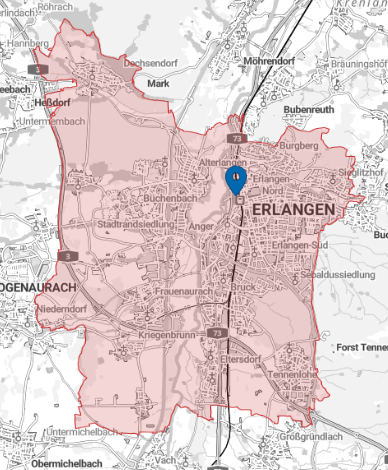
\includegraphics[width=3cm]{images/Karte_ESTW.png}
   \end{textblock*}
   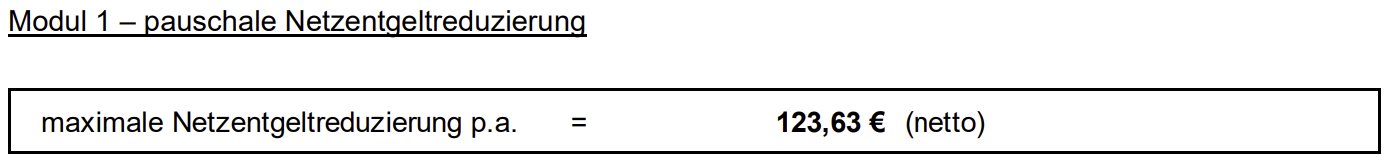
\includegraphics[width=8cm]{images/ESTW-Modul1.png}
   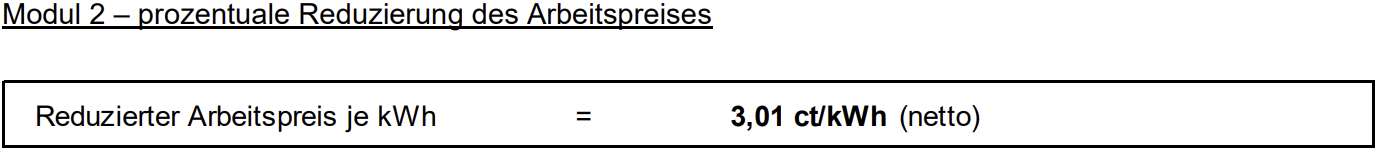
\includegraphics[width=8cm]{images/ESTW-Modul2.png}
   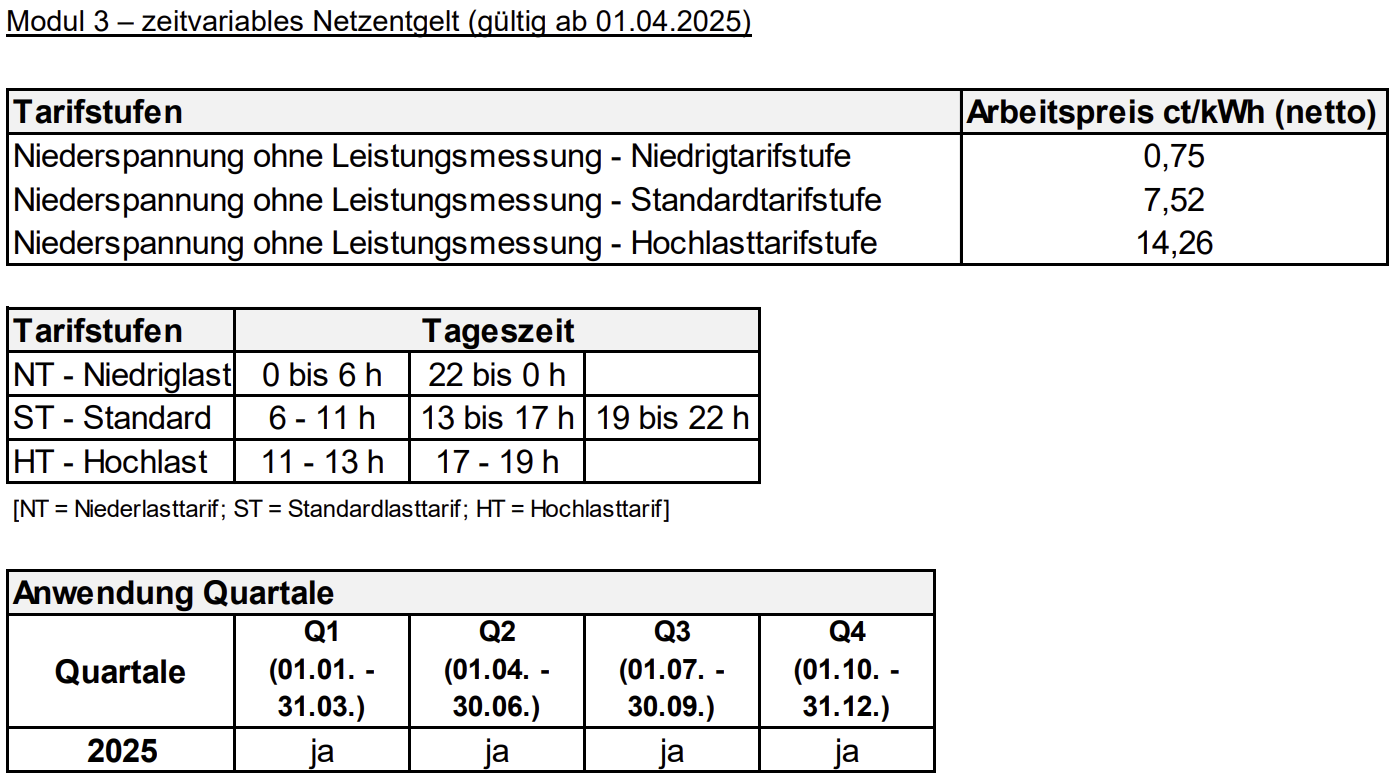
\includegraphics[width=8cm]{images/ESTW-Modul3.png}
\end{frame}

\begin{frame}{Bayernwerk}
   \begin{textblock*}{3.3cm}(9.4cm,2cm)
      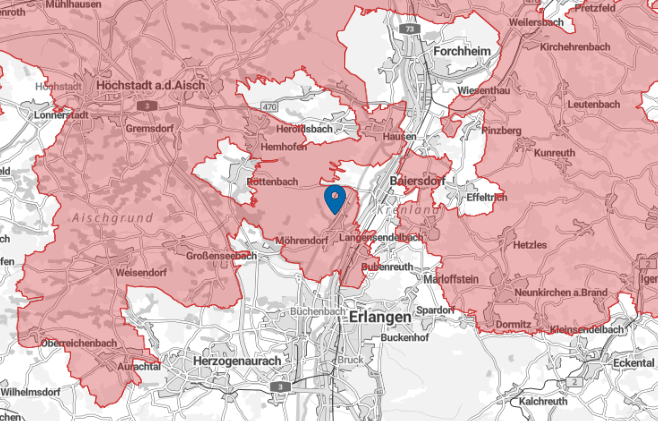
\includegraphics[width=3cm]{images/Karte_Bayernwerk.png}
   \end{textblock*}
   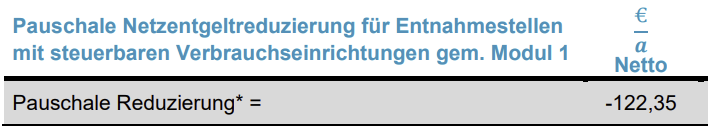
\includegraphics[width=5cm]{images/Bayernwerk-Modul1.png}
   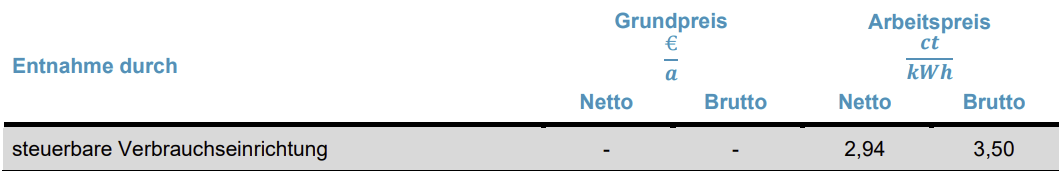
\includegraphics[width=7cm]{images/Bayernwerk-Modul2.png}
   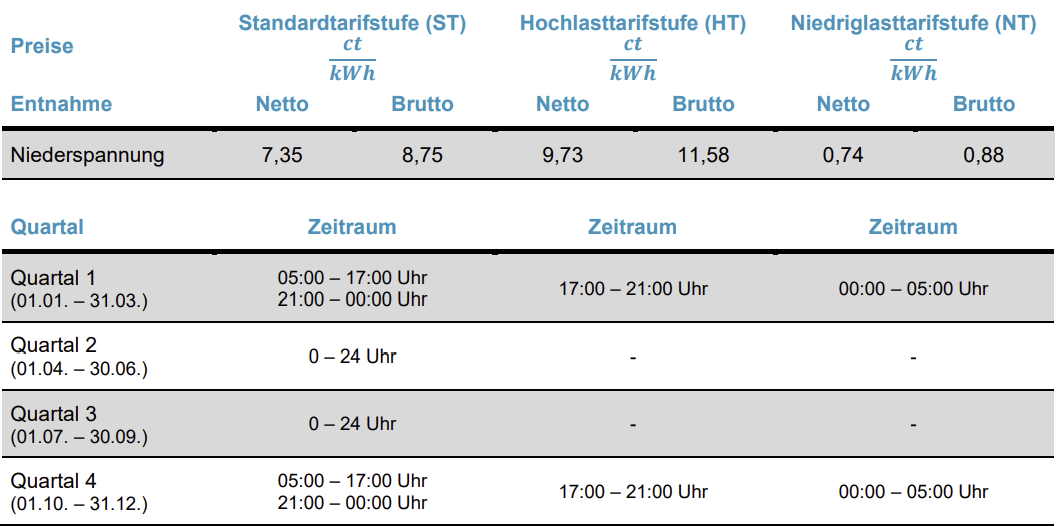
\includegraphics[width=9cm]{images/Bayernwerk-Modul3.png}
\end{frame}

\begin{frame}{Herzowerke}
   \begin{textblock*}{3.3cm}(9.4cm,2cm)
      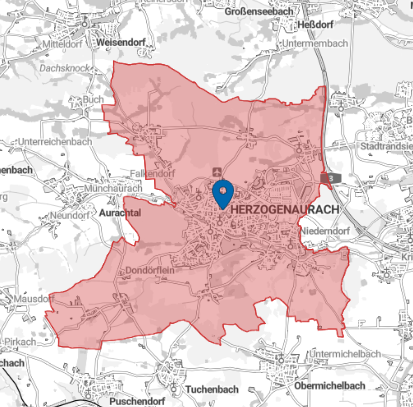
\includegraphics[width=3cm]{images/Karte_Herzowerke.png}
   \end{textblock*}
   \vspace{1.1cm}
   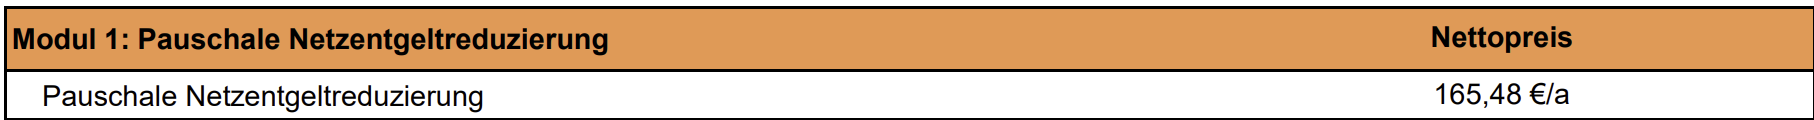
\includegraphics[width=9cm]{images/HerzoWerke-Modul1.png}
   \vspace{0.2cm}
   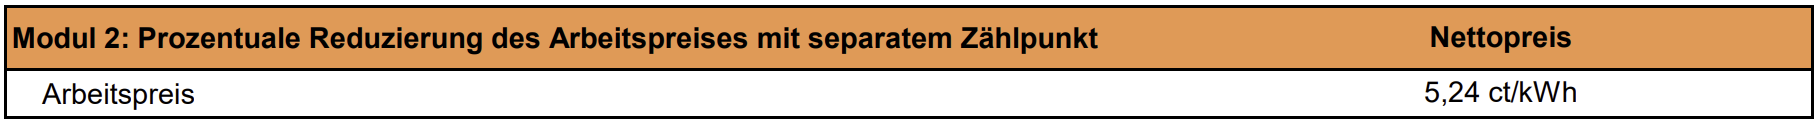
\includegraphics[width=9cm]{images/HerzoWerke-Modul2.png}
   \vspace{0.2cm}
   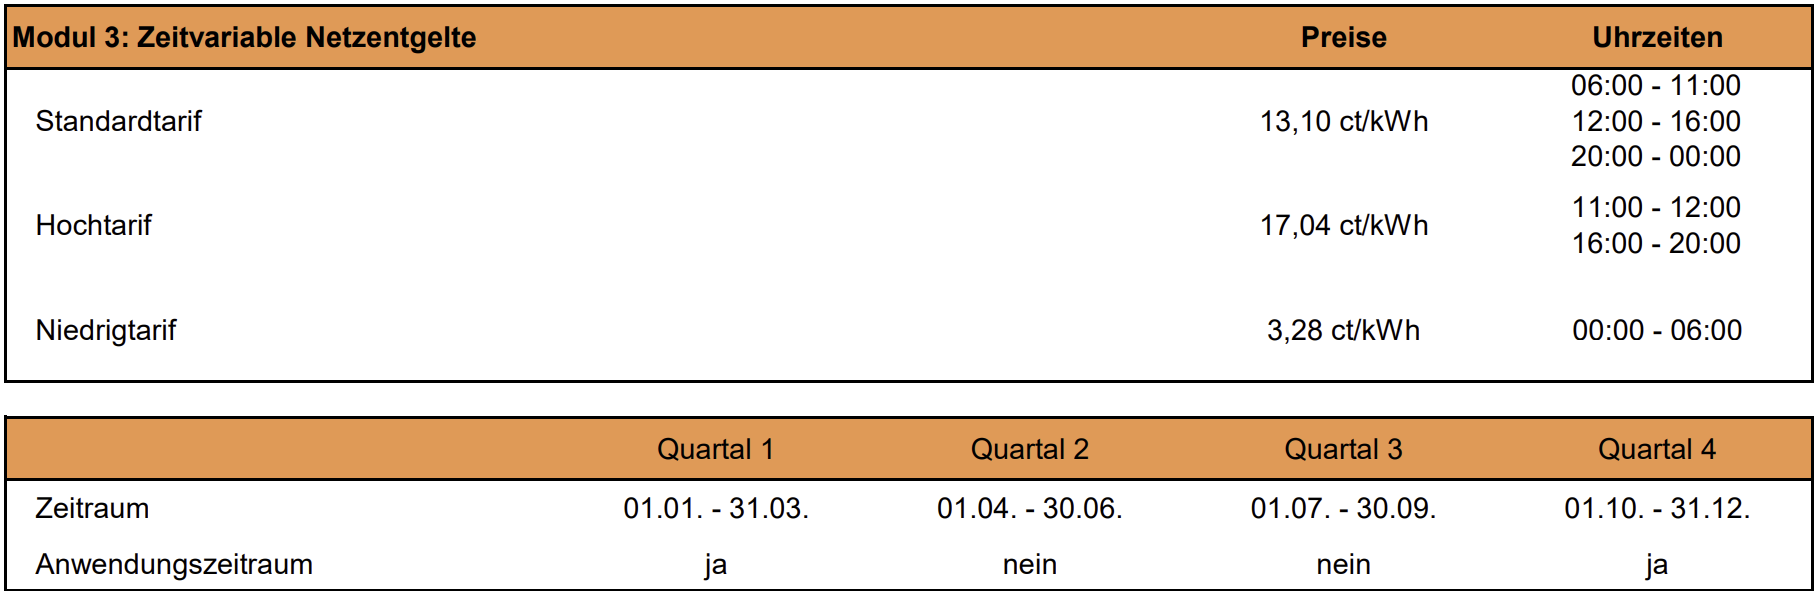
\includegraphics[width=11cm]{images/HerzoWerke-Modul3.png}
\end{frame}

\begin{frame}{N-ERGIE}
   \begin{textblock*}{3.3cm}(9.4cm,2cm)
      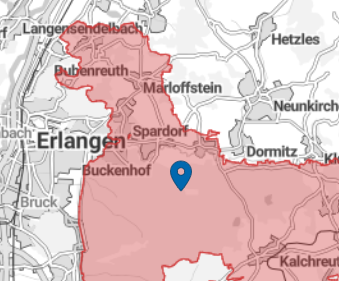
\includegraphics[width=3cm]{images/Karte_N-ERGIE.png}
   \end{textblock*}   
   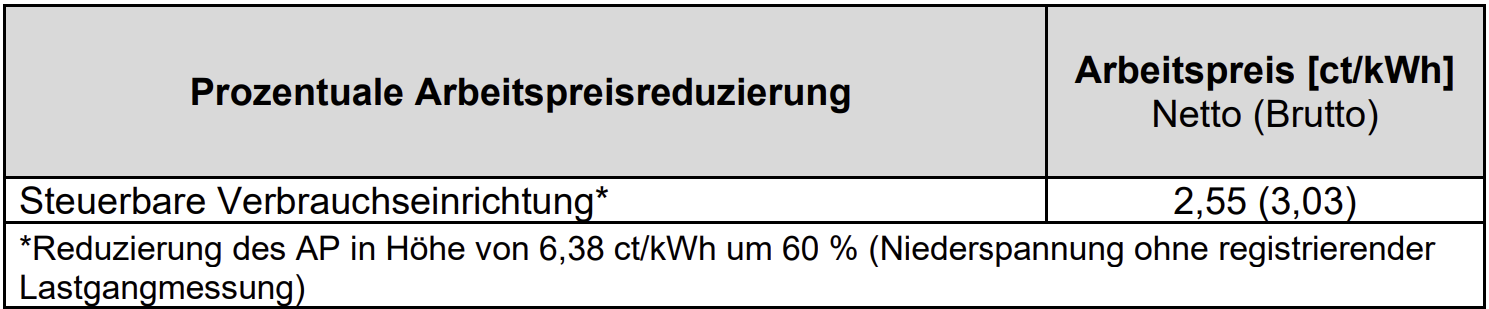
\includegraphics[width=7cm]{images/N-ERGIE-Modul1.png}
   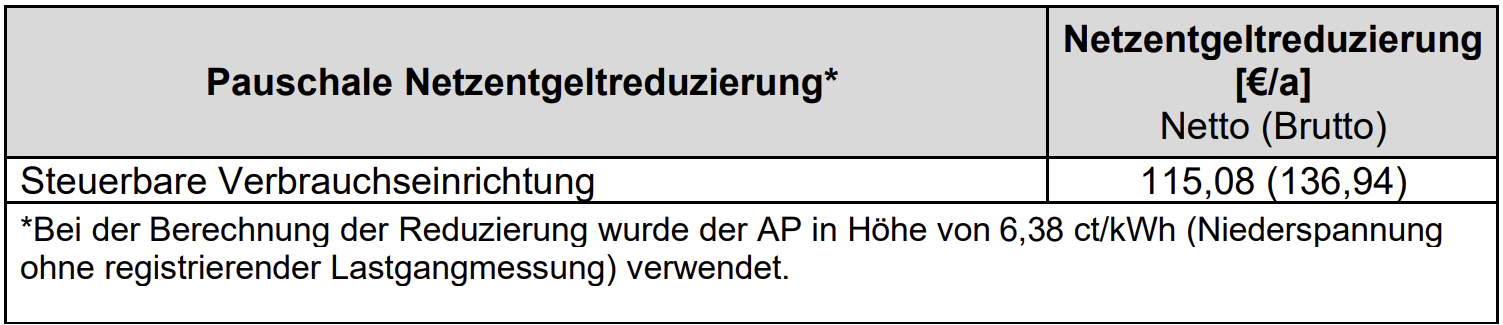
\includegraphics[width=7cm]{images/N-ERGIE-Modul2.png}
   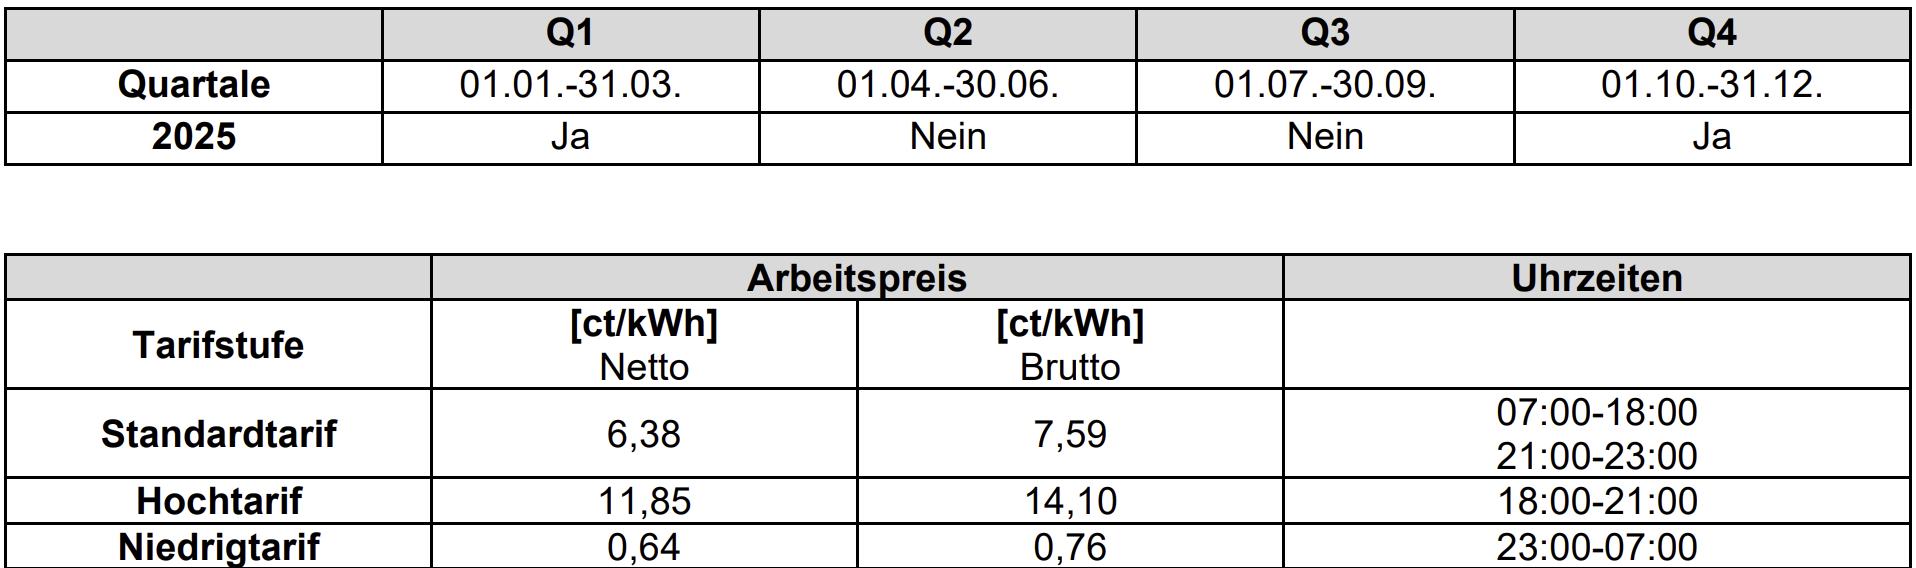
\includegraphics[width=10cm]{images/N-ERGIE-Modul3.png}
\end{frame}   

\begin{frame}{Stadtwerke Ebermannstadt}
   \begin{textblock*}{3.3cm}(9.4cm,2cm)
      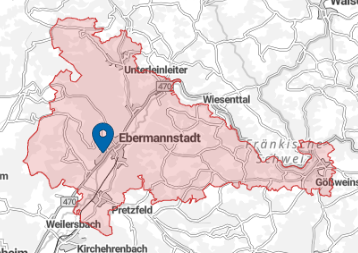
\includegraphics[width=3cm]{images/Karte_Ebermannstadt.png}
   \end{textblock*}
   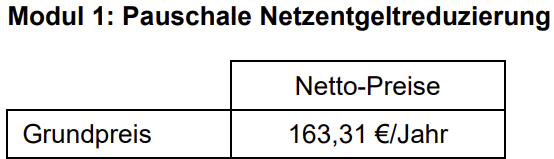
\includegraphics[width=5.5cm]{images/Ebermannstadt-Modul1.png}\\
   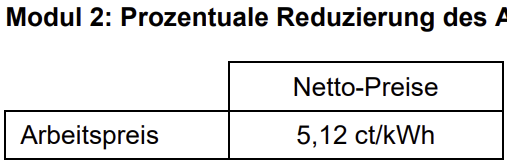
\includegraphics[width=5cm]{images/Ebermannstadt-Modul2.png}
   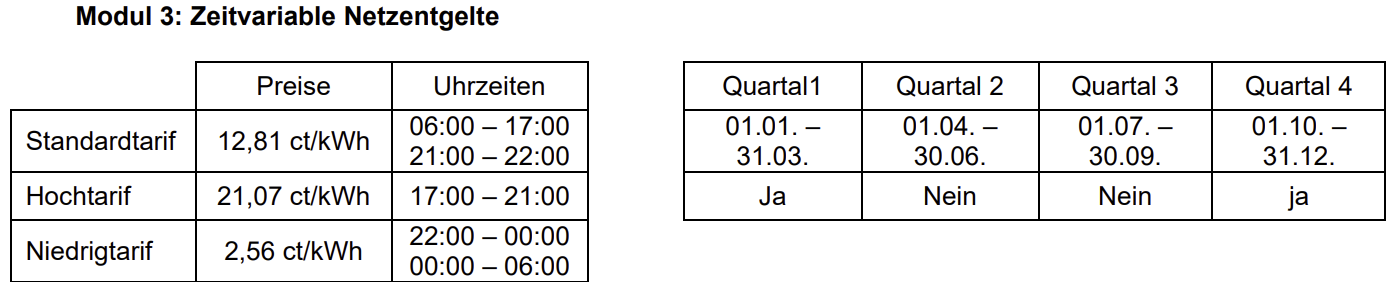
\includegraphics[width=11cm]{images/Ebermannstadt-Modul3.png}
\end{frame}

\begin{frame}{Stadtwerke Forchheim}
   \begin{textblock*}{3.3cm}(9.4cm,2cm)
      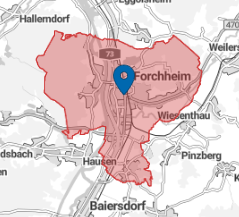
\includegraphics[width=3cm]{images/Karte_Forchheim.png}
   \end{textblock*}
   \vspace{0.6cm}
   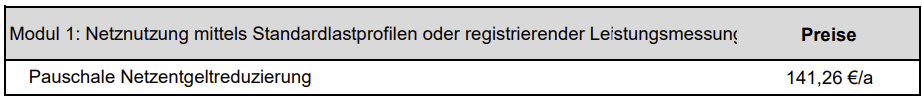
\includegraphics[width=8cm]{images/Forchheim-Modul1.png}
   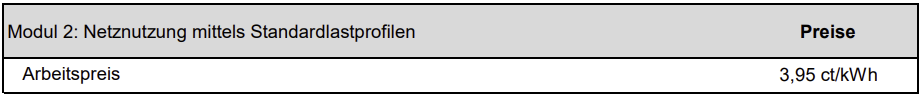
\includegraphics[width=8cm]{images/Forchheim-Modul2.png}
   \vspace{0.6cm}
   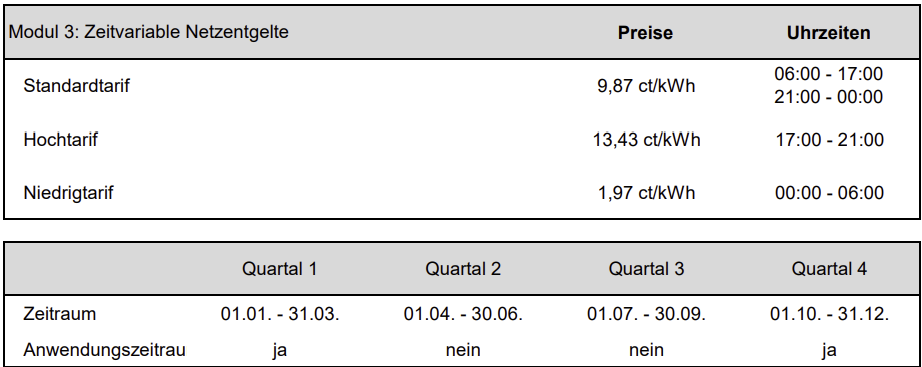
\includegraphics[width=10cm]{images/Forchheim-Modul3.png}
\end{frame}

\begin{frame}{Stadtwerke Cobug - SÜC}
   \begin{textblock*}{3.3cm}(9.4cm,2cm)
      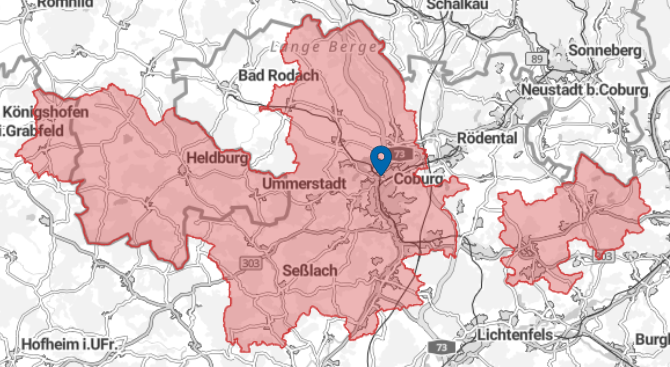
\includegraphics[width=3cm]{images/Karte_Suec.png}
   \end{textblock*}
   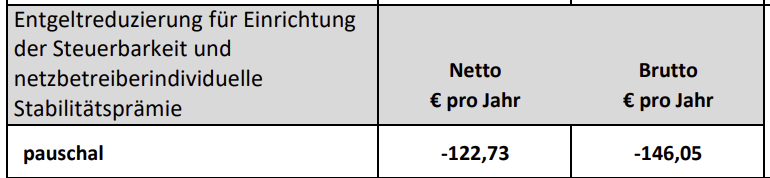
\includegraphics[width=5cm]{images/SUeC-Modul1.png}
   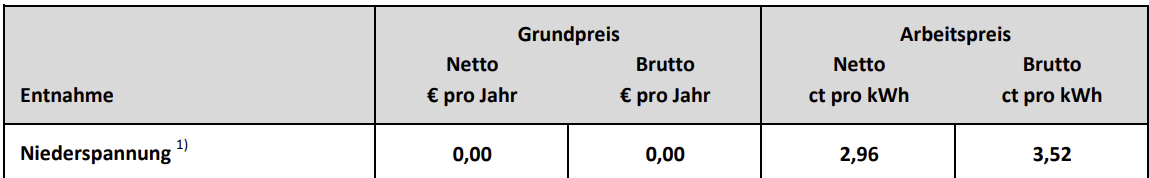
\includegraphics[width=7cm]{images/SUeC-Modul2.png}
   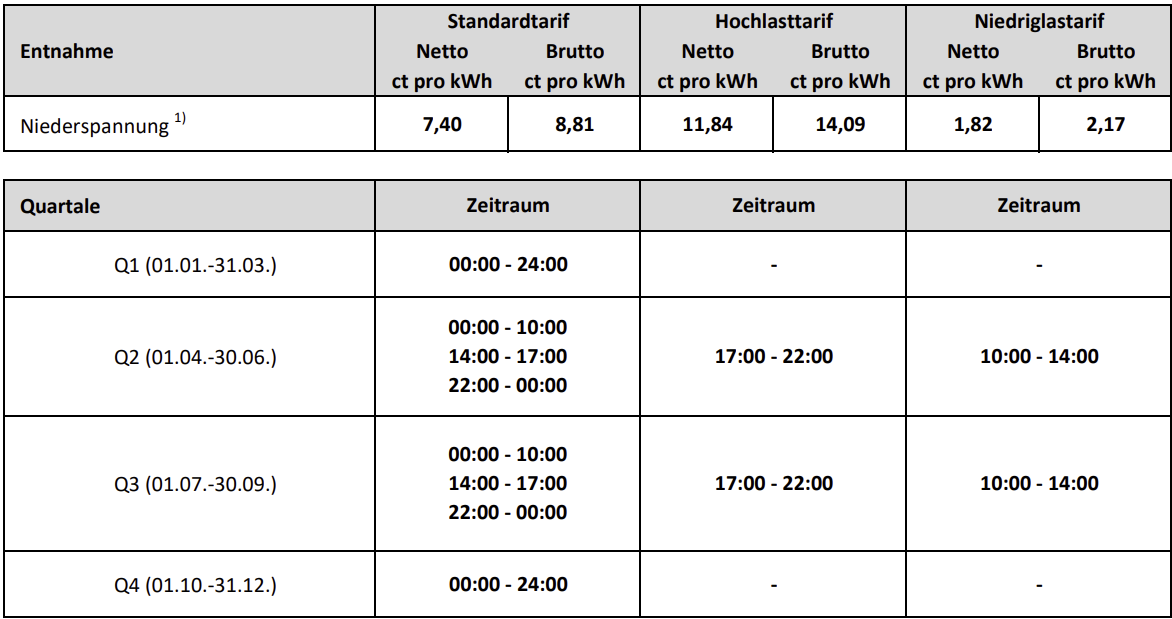
\includegraphics[width=8cm]{images/SUeC-Modul3.png}
\end{frame}

%%%%%%%%%%%%%%%%%%%%%%%%%%%
% Und jetzt?              %
%%%%%%%%%%%%%%%%%%%%%%%%%%%
\section{Und jetzt?}

\begin{frame}{Fazit, das große \enquote{ABER}!!! Und ich? $\rightarrow$ 42}
   \begin{block}{Das Salz in der Suppe}
       \begin{itemize}
           \item iMSys + CLS kosten etwas mehr (\enquote{frisst} Modul 1)
           \item PV-Anlage kann den Spaß verderben (wenn VNE in Q2 \& Q3)
           \item Manche Versorger stemmen sich dagegen (2 Quartale)
       \end{itemize}
   \end{block}

   \begin{block}{Das \enquote{Richtige} für mich?}
       \begin{description}
           \item[Modul 1] praktisch immer empfehlenswert
           \item[Modul 2] für einzelne große Verbraucher interessant (WP, BEV)
           \item[Modul 1+3] im Winter gut für WP mit Speicher(masse)
           \item[Modul 1+3] im Winter auch gut mit PV (Speicher im Winter nutzen)
           \item[Modul 1+3] im Sommer ohne PV und mit (großer) Klimaanlage
           \item[Modul 1+3] wenn Verschiebungspotenzial vorhanden
       \end{description}
   \end{block}
   \vspace{0.3cm}
\end{frame}

\begin{frame}{Und jetzt?}
   \begin{block}{Ausblick}
      \begin{itemize}
         \item Zunehmende Anzahl steuerbarer Verbraucher
         \item Einsparrechner mit Datenbank zu Netzentgelten (geplant)
         \item ...ähnlich wie der \href{https://waermepumpenrechner.streamlit.app/}{Wärmepumpenrechner}
      \end{itemize}
   \end{block}

   \vspace{0.5cm}
   \begin{block}{Weiterführende Information}
      \begin{itemize}
         \item Hager Tipp 54\cite{HagerTipp54_2024} zu §14a
         \item Energiewirtschaft einfach \href{https://www.youtube.com/watch?v=N_o7TpAXCUA}{Youtube-Video}
         \item ESTW Allg. Bedingungen ... steuerbare Verbrauchseinrichtungen\cite{ESTW2024AllgBedstVEP14a}
         \item ESTW \href{https://netze.estw.de/de/Checkliste-fuer-Anfragen-zu-Hausanschluessen/Checkliste-fuer-Anfragen-zu-Hausanschluessen.html}{Checkliste für Anfr. zu Hausanschl.} (aktuell wenig hilfreich)
      \end{itemize}
   \end{block}
\end{frame}

\usebackgroundtemplate{%
   \transparent{0.2}%
   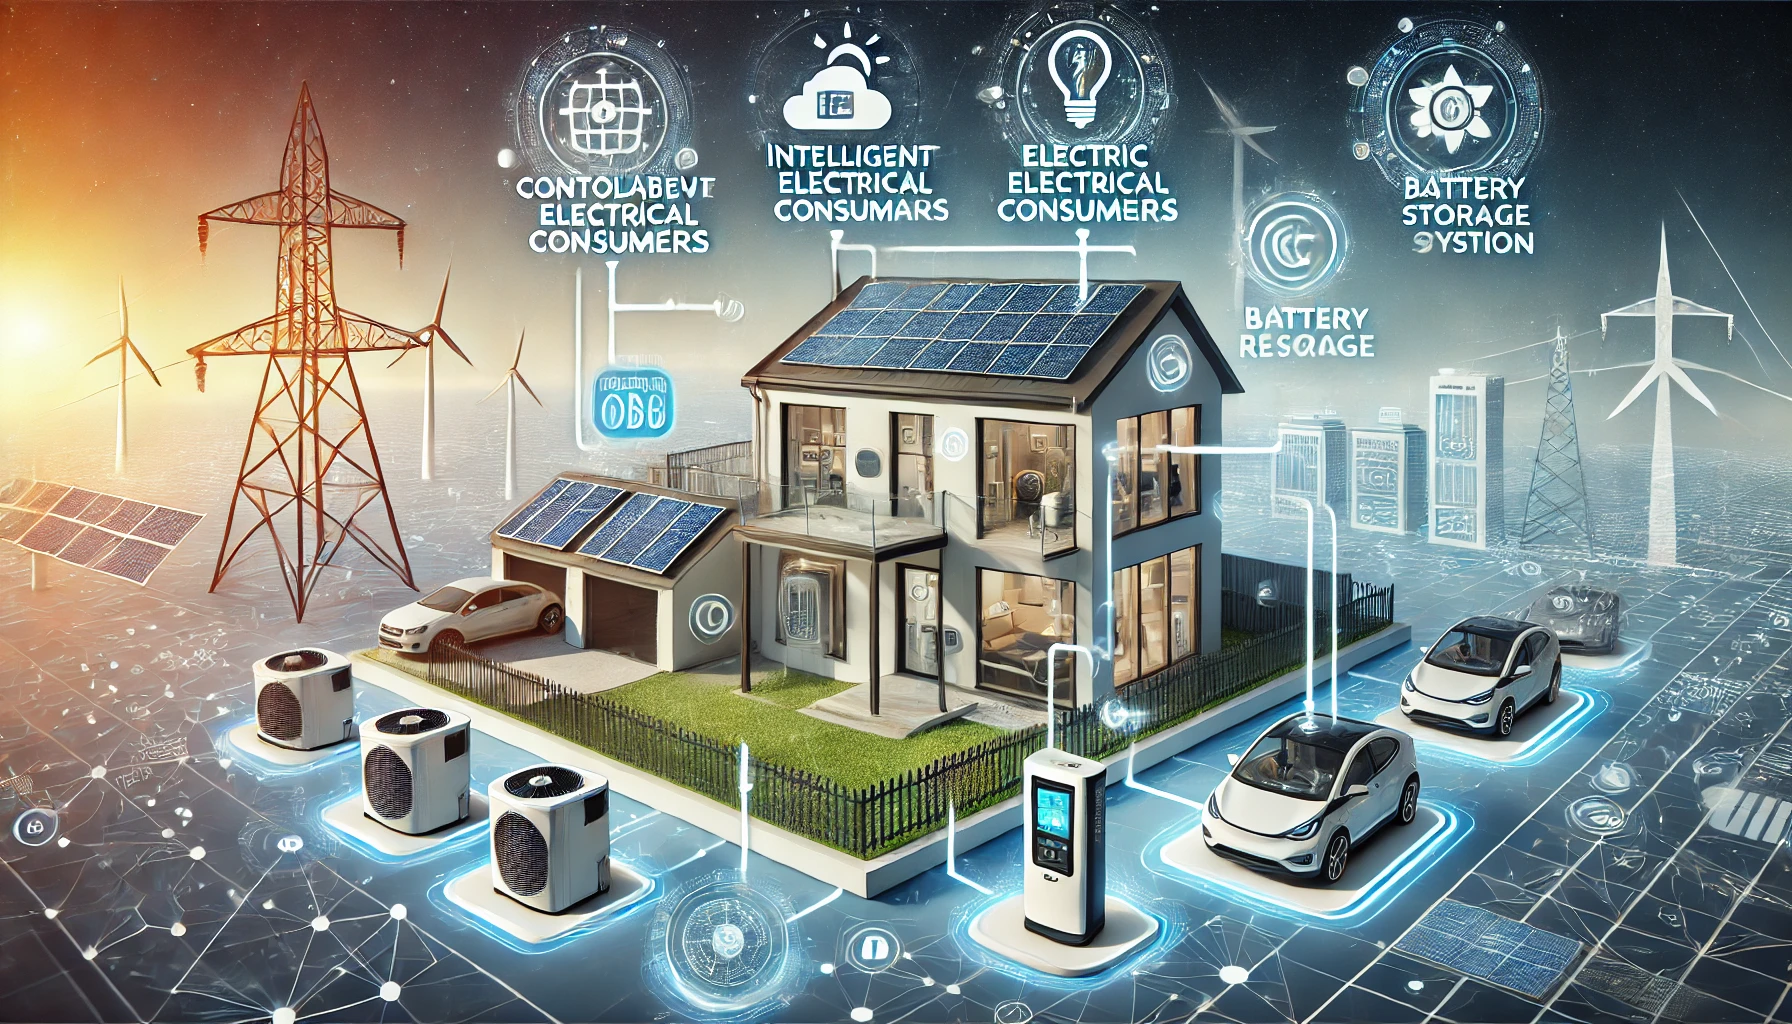
\includegraphics[width=1.05\paperwidth,viewport=0 -100 1600 1200]{images/Steuerbare_Verbraucher_2.png}%
}

\begin{frame}{Vielen Dank!}
   % Vereinslogo in der rechten oberen Ecke

   \begin{textblock*}{3cm}(0.8cm,2.2cm)  % Position (x,y) in cm anpassen
      
\includegraphics[width=3cm]{images/Logo_EWERH_eV_small.png}
   \end{textblock*}
   \vspace{1.8cm}
   \begin{center}
      \Huge Fragen?
   \end{center}
   \vfill
   \begin{minipage}{0.20\textwidth}
      \centering
      \begin{tikzpicture}
         \clip (0,0) circle (1cm);
         \node at (0,0) {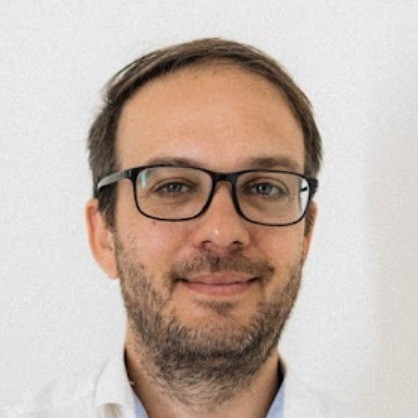
\includegraphics[width=2cm]{images/daniel_profil.jpeg}};
      \end{tikzpicture}
   \end{minipage}
   \hfill
   \begin{minipage}{0.75\textwidth}
      \begin{flushright}
         \footnotesize Daniel Glaser (Schatzmeister) \\
         \href{mailto:daniel.glaser@energiewende-erlangen.de}{daniel.glaser@energiewende-erlangen.de}
      \end{flushright}
   \end{minipage}%

   \begin{textblock*}{11cm}(0.8cm,8.7cm)
      \centering 
      \footnotesize Quelle: \url{https://github.com/the78mole/Presentation_Paragraph_14_a}
   \end{textblock*}
\end{frame}

\usebackgroundtemplate{}

% Referenzen
\begin{frame}[allowframebreaks]{Quellenverzeichnis}
   %\bibliography{references.bib}
   %\bibliographystyle{plain}
   \begingroup
      \renewcommand{\bibfont}{\scriptsize} % Verkleinert den Text der Bibliographie
      \printbibliography[heading=none]
   \endgroup
\end{frame}

\end{document}
